%definira klasu dokumenta 
\documentclass[12pt]{report} 

%prostor izmedu naredbi \documentclass i \begin{document} se zove uvod. U njemu se nalaze naredbe koje se odnose na cijeli dokument

%osnovni LaTex ne može riješiti sve probleme, pa se koriste različiti paketi koji olakšavaju izradu željenog dokumenta
\usepackage[croatian]{babel} 
\usepackage{amssymb}
\usepackage{amsmath}
\usepackage{txfonts}
\usepackage{mathdots}
\usepackage{titlesec}
\usepackage{array}
\usepackage{lastpage}
\usepackage{etoolbox}
\usepackage{tabularray}
\usepackage{color, colortbl}
\usepackage{adjustbox}
\usepackage{geometry}
\usepackage[classicReIm]{kpfonts}
\usepackage{hyperref}
\usepackage{fancyhdr}

\usepackage{float}
\usepackage{setspace}
\restylefloat{table}


\patchcmd{\chapter}{\thispagestyle{plain}}{\thispagestyle{fancy}}{}{} %redefiniranje stila stranice u paketu fancyhdr

%oblik naslova poglavlja
\titleformat{\chapter}{\normalfont\huge\bfseries}{\thechapter.}{20pt}{\Huge}
\titlespacing{\chapter}{0pt}{0pt}{40pt}


\linespread{1.3} %razmak između redaka

\geometry{a4paper, left=1in, top=1in,}  %oblik stranice

\hypersetup{ colorlinks, citecolor=black, filecolor=black, linkcolor=black,	urlcolor=black }   %izgled poveznice


%prored smanjen između redaka u nabrajanjima i popisima
\newenvironment{packed_enum}{
	\begin{enumerate}
		\setlength{\itemsep}{0pt}
		\setlength{\parskip}{0pt}
		\setlength{\parsep}{0pt}
	}{\end{enumerate}}

\newenvironment{packed_item}{
	\begin{itemize}
		\setlength{\itemsep}{0pt}
		\setlength{\parskip}{0pt}
		\setlength{\parsep}{0pt}
	}{\end{itemize}}




%boja za privatni i udaljeni kljuc u tablicama
\definecolor{LightBlue}{rgb}{0.9,0.9,1}
\definecolor{LightGreen}{rgb}{0.9,1,0.9}

%Promjena teksta za dugačke tablice
\DefTblrTemplate{contfoot-text}{normal}{Nastavljeno na idućoj stranici}
\SetTblrTemplate{contfoot-text}{normal}
\DefTblrTemplate{conthead-text}{normal}{(Nastavljeno)}
\SetTblrTemplate{conthead-text}{normal}
\DefTblrTemplate{middlehead,lasthead}{normal}{Nastavljeno od prethodne stranice}
\SetTblrTemplate{middlehead,lasthead}{normal}

%podesavanje zaglavlja i podnožja

\pagestyle{fancy}
\lhead{Programsko inženjerstvo}
\rhead{Što želiš čitati?}
\lfoot{DaVincijevi koderi}
\cfoot{stranica \thepage/\pageref{LastPage}}
\rfoot{\today}
\renewcommand{\headrulewidth}{0.2pt}
\renewcommand{\footrulewidth}{0.2pt}


\begin{document} 
	
	
	
	\begin{titlepage}
		\begin{center}
			\vspace*{\stretch{1.0}} %u kombinaciji s ostalim \vspace naredbama definira razmak između redaka teksta
			\LARGE Programsko inženjerstvo\\
			\large Ak. god. 2023./2024.\\
			
			\vspace*{\stretch{3.0}}
			
			\huge Što želiš čitati?\\
			\Large Dokumentacija, Rev. \textit{1}\\
			
			\vspace*{\stretch{12.0}}
			\normalsize
			Grupa: \textit{DaVincijevi koderi}\\
			Voditelj: \textit{Andrea Gazibarić}\\
			
			
			\vspace*{\stretch{1.0}}
			Datum predaje: \textit{17.11.2023.}\\
	
			\vspace*{\stretch{4.0}}
			
			Nastavnik: \textit{Alan Jović}\\
		
		\end{center}

	
	\end{titlepage}

	
	\tableofcontents


	\chapter{Dnevnik promjena dokumentacije}
		
				
		
		\begin{longtblr}[
				label=none
			]{
				width = \textwidth, 
				colspec={|X[2]|X[13]|X[3]|X[3]|}, 
				rowhead = 1
			}
			\hline
			\textbf{Rev.}	& \textbf{Opis promjene/dodatka} & \textbf{Autori} & \textbf{Datum}\\[3pt] \hline
			0.1 & Napravljen predložak.	& * & 26.10.2023. 		\\[3pt] \hline  
			0.2	& Dodani funkcionalni zahtjevi, aktori i dionici. & * & 27.10.2023. 	\\[3pt] \hline 
			0.2.1 & Ispravak funkcionalnih zahtjeva. & * & 28.10.2023. 	\\[3pt] \hline
			0.2.2	& Dodan opis funkcionalnih zahtjeva. & * & 30.10.2023. 	\\[3pt] \hline
			0.2.3	& Ispravak opisa funkcionalnih zahtjeva. & * & 02.11.2023. 	\\[3pt] \hline
			0.2.4	& Dodani dijagrami obrazaca uporabe. & * & 02.11.2023. 	\\[3pt] \hline
			0.3	& Dodani ER i REL dijagrami baze podataka. & * & 02.11.2023. 	\\[3pt] \hline
			0.4 & Dodani sekvencijski dijagrami. & * & 05.11.2023. \\[3pt] \hline 
			0.4.1 & Dodan opis sekvencijskih dijagrama. & * & 06.11.2023. \\[3pt] \hline
			0.5 & Arhitektura i dizajn sustava, algoritmi i strukture podataka. & * & .11.2023. \\[3pt] \hline 
			0.6	& Dodan opis nefunkcionalnih zahtjeva. & * & .11.2023. 	\\[3pt] \hline
			0.7	& Dodan opis projektnog zadatka. & * & .11.2023. 	\\[3pt] \hline 
			0.8 & Dodani dijagrami razreda. & * & .11.2023. \\[3pt] \hline 
			\textbf{1.0} & Verzija samo s bitnim dijelovima za 1. ciklus. & * & .11.2023. \\[3pt] \hline  
			&  &  & \\[3pt] \hline	
		\end{longtblr}
		
	\chapter{Opis projektnog zadatka}
		
		\textbf{\textit{dio 1. revizije}}\\
		 Cilj ovog projekta je razviti programsku podršku za stvaranje web aplikacije  ” Što želiš čitati?” kojoj je glavni zadatak omogućiti korisniku pronalazak ponuditelja knjige u blizini koji ima u prodaji traženu knjigu na hrvatskom ili srodnom jeziku. Te omogućuje i međusobno povezivanje ponuditelja knjiga radi proširenja međusobnih ponuda. Naime ljubitelji čitanja koji žele čitati stranu literaturu imaju problem s pronalaskom željenih knjiga na hrvatskom zato što mnogi naslovi nisu prevedeni na hrvatski ili srodni jezik poput srpskog i bosanskog, a u slučaju da postoji prijevod zbog loše ažurnosti web stranica ponuditelja knjiga nije ih lako pronaći.  

        Stoga je ideja ove web aplikacije da omogući čitatelju unos značajke željene knjige, imena i ili ponuditelja knjige te pretraga dostupnosti po navedenim značajkama.  Potencijalna korist ovog projekta je što olakšava i ubrzava čitateljima pronalazak tražene knjige, a u slučaju da one ne postoji ne oduzima im puno vremena, te tako poboljšava njihovo čitalačko iskustvo.  Dodatna potencijalna korist je što čitatelju omogućava proširivanje horizonata i upoznavanje sa stranom kulturom čitajući stranu literaturu. Rezultat toga bi bila promocija kulture čitanja na području Republike Hrvatske. S druge strane, ponuditelji knjiga, poput izdavača, antikvarijata i preprodavača, imaju priliku proširiti svoj doseg na širu publiku te povećavajući prodaju knjiga iz svoje ponude. To pomoglo malim poduzetnicima koji drže antikvarijate i nezavisne knjižare da ostanu u poslu, a osnažilo bi izdavače  da prošire svoju ponudu i prevedu još i više stranih naslova, te bi samim time i kupci bili zadovoljniji. 

        U aplikaciji postoje tri uloge:
        \begin{packed_item}
			\item \textit{Neregistrirani korisnik: potraživač knjiga, kupac}
			\item \textit{Registrirani korisnik: ponuditelj knjiga}
			\item \textit{Administrator }
		\end{packed_item}
        Neregistrirani korisnik ima mogućnost pristupu web sjedištu aplikacije, te može pretraživati ponude knjiga. Pretraga se provodi po značajkama knjige koju koje neregistrirani korisnik unosi i po nazivu ponuditelja. Neregistriranom korisniku se nudi pregled karte na kojoj su označene lokacije (adrese) svih ponuditelja knjiga te ih on može izabrati. Nakon odabira ponuditelja neregistriranom korisniku prikazuje se popis, to jest ponuda svih knjiga izabranog ponuditelja. Ponuđene knjige sadržavaju sljedeće značajke:
        \begin{packed_item}
			\item \textit{naziv,}
			\item \textit{autore,}
			\item \textit{godinu izdanja,}
			\item \textit{izdavača,}
			\item \textit{kategorija izdavača (domaći, strani),}
			\item \textit{žanr,}
            \item \textit{ISBN,}
			\item \textit{broj izdanja,}
			\item \textit{stanje očuvanosti,}
			\item \textit{tekstni opis,}
			\item \textit{sliku korica,}
			\item \textit{oznaku vrste knjige,}
            \item \textit{listu ponuda.}
		\end{packed_item}
        S time da oznaku vrste knjige možemo okarakterizirati u 5 različitih kategorija:
        \begin{packed_item}
			\item \textit{Knjiga je na stranom jeziku (npr. engleski), a ne postoji izdanje na hrvatskom ili srodnom jeziku (bosanski, srpski) }
			\item \textit{Knjiga je izdana na hrvatskom jeziku i dobavljiva je na području Hrvatske}
			\item \textit{Knjiga je izdana na hrvatskom jeziku, ali nije dobavljiva na području Hrvatske (npr. izdavač je rasprodao izdanje)}
			\item \textit{Knjiga je izdana na srodnom jeziku, dobavljiva je samo na njihovom tržištu }
			\item \textit{Knjiga je izdana na srodnom jeziku, dobavljiva je u Hrvatskoj, ne postoji na hrvatskom jeziku}
		\end{packed_item}
        Dok lista ponude svake knjige treba uključivati:
        \begin{packed_item}
			\item \textit{naziv ponuditelja,}
			\item \textit{broj dostupnih primjeraka,}
			\item \textit{cijenu knjige kod dotičnog ponuditelja.}
		\end{packed_item}
        Uz to da ako knjiga nema više dostupnih registriranih  ponuditelja knjigu se ne prikazuje u ponudi prilikom pretrage u sustavu.
        Osim odabira ponuditelja i pretrage ponuđenih knjiga, neregistriranom korisniku se daje i mogućnost da kroz sučelje aplikacije zatraži od registriranog korisnika izdavača da stavi u ponudu prijevod željene knjige i samim time u dogovoru sa stranim izdavačem prevede knjigu na hrvatski jezik. Zahtjevi za prijevod se jednostavno bilježe na stranici i akumuliraju se za svaku knjigu na stranom jeziku kako bi ponuditelj imao uvid o potražnji prijevoda. Važno je još napomenuti da ostala komunikacija vezana uz nabavu knjige između neregistriranog korisnika i ponuditelja se ne odvaja kroz aplikaciju već preko drugih kanala poput e-pošte i telefonskim pozivom. 
        
        Registrirani korisnik je isključivo ponuditelj knjiga koji spada u jednu od tri kategorije:
        \begin{packed_item}
			\item \textit{Izdavač}
			\item \textit{Antikvarijat}
			\item \textit{Preprodavač}
		\end{packed_item}
        Ponuditelj bira svoju kategoriju tijekom registracije, pri čemu registraciju treba odobriti administrator nakon pregleda zahtjeva. Nadalje registrirani korisnik unosi potrebne informacije za kontakt ponuditelja, a to su: 
        \begin{packed_item}
			\item \textit{naziv,}
			\item \textit{e-pošta,}
			\item \textit{adresa,}
			\item \textit{izdavača,}
			\item \textit{broj telefona.}
		\end{packed_item}
        Nakon toga registrirani korisnik pristupa web aplikaciji uz pomoć korisničkog imena i lozinke. Svaki ponuditelj ima mogućnost ponuditi neograničeni broj naslova knjiga i njezinih primjeraka u skladu sa svojom kategorijom. Tijekom kreiranja ponude svaki ponuditelj je primoran ispravno odrediti oznaku vrste knjige, te pri svakom dodavanju nove knjige ili primjeraka već postojeće knjige u web aplikaciju. Uz to pri svakoj izmjeni ponude knjiga poput dodavanja novih primjeraka već postojeće knjige ili uklanjanju primjeraka koji su prodani ponuditelj je dužan provjeriti da oznaka vrste knjige odgovara stvarnosti i ako to nije slučaj, izmijeniti ju. Ponuditelj također nije obavezan ponuditi sve knjige koje ima u ponudi, to jest u svojoj ponudi može imati više knjiga nego što ih je ponudio na web stranici.
        Izdavač u svojoj ponudi smije nuditi knjige isključivo knjige na hrvatskom jeziku, te na temelju prikupljenih zahtjeva neregistriranih korisnika smije zatražiti izdavača strane knjige za dozvolu prijevoda knjige sa stranog ili srodnog jezika na hrvatski jezik. 
        Antikvarijat u svojoj ponudi smije imati knjige na stranom jeziku, srodnom jeziku ili hrvatskom jeziku, s time da se mora svojom adresom nalaziti isključivo na području Hrvatske.
        Preprodavač u svojoj ponudi može imati sve vrste knjiga neovisno o prijevodu, te i one koje nisu na drugačiji način dobavljive na području Hrvatske. Uz to adresa mu može biti u Hrvatskoj i u zemljama sa srodnim jezikom, odnosno Srbiji i Bosni i Hercegovini.
       
        Skup korisnika koji bi mogao biti zainteresiran za ostvareno rješenje se može raščlaniti na četiri skupa:
        \begin{packed_item}
			\item \textit{Ljubitelji knjiga: Oni koji traže stranu literaturu prevedene na hrvatski jezik ili srodne jezike.}
			\item \textit{Izdavači: Oni koji žele proširiti dostupnost svojih knjiga na novo tržište.}
			\item \textit{Antikvarijati: Oni koji imaju rijetke ili stare knjige koje žele ponuditi zainteresiranim čitateljima i kolekcionarima.}
		\end{packed_item}
        Aplikacija bi se u budućnosti mogla proširiti na različite načine koji bi poboljšali zadovoljstvo neregistriranih i registriranih korisnika:
        U slučaju da u ponudi nema tražene knjige čitatelju bi se moglo ponuditi knjiga u ponudi od istog autora ili slične tematike, te na taj način čitatelj bi dobio štivo za čitanje, a ponuditelj bio ostvario dodatnu prodaju. 
        Mogla bi se omogući komunikacija kupca i ponuditelja unutar aplikacije kako bi se kupcu olakšala kupnja.
        Moglo bi se omogućiti neregistriranim korisnicima da uz zahtjev za prijevodom određenog naslova mogu unijeti email kako bi mogli biti obaviješteni o izlasku prijevoda i proširenju ponude.

	\chapter{Specifikacija programske potpore}
		
	\section{Funkcionalni zahtjevi}
			
			
			\noindent \textbf{Dionici:}
			\begin{packed_enum}
				\item Neregistrirani korisnici
				\item Registrirani korisnici
					\begin{packed_enum}
						\item Izdavači
						\item Antikvarijati
						\item Preprodavači
					\end{packed_enum}
				\item Administratori
				\item Baza podataka
			\end{packed_enum}
			
			\noindent \textbf{Aktori i njihovi funkcionalni zahtjevi:}
			\begin{packed_enum}
			
				\item  \underbar{Neregistrirani korisnik (inicijator) može:}
				\begin{packed_enum}
					\item pretraživati ponudu knjiga po:
					\begin{packed_enum}
						\item  značajkama knjige 
						\item  ponuditelju
					\end{packed_enum}
					\item  pretraživati ponuditelje na karti
					\item odabrati ponuditelja i izlistati sve knjige u njegovoj ponudi
					\item zahtjevati od izdavača da kontaktira stranog izdavača za prijevod
					\item registrirati se 
						\begin{packed_item}
							\item unijeti podatke
						\end{packed_item}
				\end{packed_enum}
			
				\item  \underbar{Izdavač (inicijator) može:}
				\begin{packed_enum}
					\item zatražiti od stranog izdavača dozvolu za prijevod
					\item ponuditi knjige na hrvatskom jeziku
					\item maknuti knjige iz svoje ponude
				\end{packed_enum}
				
				\item  \underbar{Antikvarijat (inicijator) može:}
				\begin{packed_enum}
					\item ponuditi knjige na hrvatskom i srodnim jezicima
					\item maknuti knjige iz svoje ponude
				\end{packed_enum}
				
				\item  \underbar{Preprodavač (inicijator) može:}
				\begin{packed_enum}
					\item ponuditi knjige na bilo kojem jeziku
					\item maknuti knjige iz svoje ponude
				\end{packed_enum}
								
				\item \underbar{Administrator (inicijator) može:}
					\begin{packed_enum}
						\item odobriti registraciju
							\begin{packed_item}
								\item provjeriti je li adresa antikvarijata u RH i 
								\item jesu li ostali podatci dobri
							\end{packed_item}
						\item ukloniti registrirane korisnike
						\item mijenjati vrstu korisnika
						\item pristupiti bazi podataka
					\end{packed_enum}
					
				\item \underbar{Baza podataka (sudionik) pohranjuje podatke o:}
					\begin{packed_enum}
						\item registriranim korisnicima
						\item knjigama (uključujući i oznake knjige)
						\item zahtjevima za prijevod
					\end{packed_enum}
					
			\end{packed_enum}
			
			\eject 
			
			
				
			\subsection{Obrasci uporabe}
			
					\noindent \textbf{Opis obrazaca uporabe} \\
					

					\noindent \underbar{\textbf{UC1 - Pretraživanje knjiga po značajkama}}
					\begin{packed_item}
						\item \textbf{Glavni sudionik: }Neregistrirani korisnik
						\item  \textbf{Cilj:} Pregledati ponudu knjiga
						\item  \textbf{Sudionici:} Baza podataka
						\item  \textbf{Preduvjet:} -
						\item  \textbf{Opis osnovnog tijeka:}
						\item[] \begin{packed_enum}
							\item odabir značajki knjige po kojima se želi pretražiti
							\item prikazuje se ponuda knjiga s odabranim značajkama
						\end{packed_enum}
					\end{packed_item}
					
					\noindent \underbar{\textbf{UC2 - Pretraživanje knjiga po ponuditelju}}
					\begin{packed_item}
						\item \textbf{Glavni sudionik: }Neregistrirani korisnik
						\item  \textbf{Cilj:} Pregledati ponudu knjiga
						\item  \textbf{Sudionici:} Baza podataka
						\item  \textbf{Preduvjet:} -
						\item  \textbf{Opis osnovnog tijeka:}
						\item[] \begin{packed_enum}
							\item odabir ponuditelja čiju ponudu želi pregledati
							\item prikazuje se ponuda knjiga odabranog poslužitelja
						\end{packed_enum}
					\end{packed_item}
					
					\noindent \underbar{\textbf{UC3 - Pretraživanje ponuditelja na karti}}
					\begin{packed_item}
						\item \textbf{Glavni sudionik: }Neregistrirani korisnik
						\item  \textbf{Cilj:} Pregledati ponuditelje u blizini
						\item  \textbf{Sudionici:} Baza podataka
						\item  \textbf{Preduvjet:} -
						\item  \textbf{Opis osnovnog tijeka:}
						\item[] \begin{packed_enum}
							\item otvaranje karte s označenim ponuditeljima
							\item odabir lokacije i ponuditelja
							\item ispis podataka o ponuditelju i njihove ponude
						\end{packed_enum}
					\end{packed_item}
					
					\noindent \underbar{\textbf{UC4 - Zahtjev za prijevodom}}
					\begin{packed_item}
						\item \textbf{Glavni sudionik: }Neregistrirani korisnik
						\item  \textbf{Cilj:} Zatražiti prijevod knjige na stranom jeziku
						\item  \textbf{Sudionici:} Izdavač, baza podataka
						\item  \textbf{Preduvjet:} Knjiga nije prevedena na hrvatski
						\item  \textbf{Opis osnovnog tijeka:}
						\item[] \begin{packed_enum}
							\item odabir ~"Zahtjevaj prijevod" u sučelju aplikacije
							\item zahtjev se bilježi u bazu podataka
							\item izdavač dobija poruku o novom zahtjevu
						\end{packed_enum}
					\end{packed_item}
					
					\noindent \underbar{\textbf{UC5 - Registracija}}
					\begin{packed_item}
						\item \textbf{Glavni sudionik: }Neregistrirani korisnik
						\item  \textbf{Cilj:} Registrirati se kao ponuditelj
						\item  \textbf{Sudionici:} Baza podataka, administrator
						\item  \textbf{Preduvjet:} -
						\item  \textbf{Opis osnovnog tijeka:}
						\item[] \begin{packed_enum}
							\item odabir "Sign up" u sučelju
							\item unos vrste ponuditelja (izdavač, antikvarijat, preprodavač)
							\item unos podataka (naziv, e-pošta, adresa, broj telefona)
							\item unos korisničkog imena i lozinke
							\item administrator odobrava račun
							\item poruka na e-pošti o odobrenju ili neodobrenju računa
						\end{packed_enum}
						\item  \textbf{Opis mogućih odstupanja:}
						\item[] \begin{packed_item}
							\item[3.a] adresa antikvarijata nije u RH
							\item[] \begin{packed_enum}
								\item nemogućnost nastavka registracije bez promjene podataka
								\item upozorenje
							\end{packed_enum}
							\item[3.b] adresa preprodavača nije u zemlji srodnog jezika
							\item[] \begin{packed_enum}
								\item nemogućnost nastavka registracije bez promjene podataka
								\item upozorenje
							\end{packed_enum}
							\item[4.a] korisničko ime već postoji
							\item[] \begin{packed_enum}
								\item nemogućnost nastavka registracije bez promjene podataka
								\item upozorenje
							\end{packed_enum}	
						\end{packed_item}
					\end{packed_item}
					
					\noindent \underbar{\textbf{UC6 - Ponuda naslova knjiga}}
					\begin{packed_item}
						\item \textbf{Glavni sudionik: }Ponuditelj
						\item  \textbf{Cilj:} Ponuditi neograničen broj naslova knjiga
						\item  \textbf{Sudionici:} Baza podataka
						\item  \textbf{Preduvjet:} Registrirati se kao ponuditelj
						\item  \textbf{Opis osnovnog tijeka:}
						\item[] \begin{packed_enum}
							\item Ponuditelj odabire ~"Ponudi naslov knjige" u sučelju aplikacije
							\item Ponuditelj odabire naslove koje želi ponuditi
							\item U bazu podataka se pohrani promjena
						\end{packed_enum}
					\end{packed_item}
					
					\noindent \underbar{\textbf{UC7 - Ponuda primjeraka knjiga}}
					\begin{packed_item}
						\item \textbf{Glavni sudionik: }Ponuditelj
						\item  \textbf{Cilj:} Ponuditi neograničen broj primjeraka knjiga
						\item  \textbf{Sudionici:} Baza podataka
						\item  \textbf{Preduvjet:} Registrirati se kao ponuditelj
						\item  \textbf{Opis osnovnog tijeka:}
						\item[] \begin{packed_enum}
							\item Ponuditelj odabire ~"Ponudi primjerak knjige" u sučelju aplikacije
							\item Ponuditelj odabire primjerke knjiga
							\item U bazu podataka se pohrani promjena
						\end{packed_enum}
					\end{packed_item}
					
					\noindent \underbar{\textbf{UC8 - Pregled želja neregistriranih korisnika}}
					\begin{packed_item}
						\item \textbf{Glavni sudionik: }Izdavač
						\item  \textbf{Cilj:} Prikupiti želje neregistriranih korisnika
						\item  \textbf{Sudionici:} Baza podataka
						\item  \textbf{Preduvjet:} Registrirati se kao izdavač
						\item  \textbf{Opis osnovnog tijeka:}
						\item[] \begin{packed_enum}
							\item Praćenje aktivnosti neregistriranog korisnika
							\item Bilježenje i prikupljanje njegovih želja
						\end{packed_enum}
					\end{packed_item}
					
					\noindent \underbar{\textbf{UC9 - Zahtjev za dozvolu prijevoda sa stranog jezika}}
					\begin{packed_item}
						\item \textbf{Glavni sudionik: }Izdavač
						\item  \textbf{Cilj:} Zatražiti prijevod knjige sa stranog jezika na hrvatski
						\item  \textbf{Sudionici:} Baza podataka
						\item  \textbf{Preduvjet:} Registrirati se kao izdavač
						\item  \textbf{Opis osnovnog tijeka:}
						\item[] \begin{packed_enum}
							\item Izdavač pregleda želje neregistriranih korisnika
							\item Izdavač odabire knjige
							\item Izdavač zatraži dozvolu za prijevodom
						\end{packed_enum}
					\end{packed_item}
					
					\noindent \underbar{\textbf{UC10 - Zahtjev za dozvolu prijevoda sa srodnog jezika}}
					\begin{packed_item}
						\item \textbf{Glavni sudionik: }Izdavač
						\item  \textbf{Cilj:} Zatražiti prijevod knjige sa srodnog jezika na hrvatski
						\item  \textbf{Sudionici:} Baza podataka
						\item  \textbf{Preduvjet:} Registrirati se kao izdavač
						\item  \textbf{Opis osnovnog tijeka:}
						\item[] \begin{packed_enum}
							\item Izdavač pregleda želje neregistriranih korisnika
							\item Izdavač odabire knjige
							\item Izdavač zatraži dozvolu za prijevodom
						\end{packed_enum}
					\end{packed_item}
					
					\noindent \underbar{\textbf{UC11 - Ponuda knjiga na hrvatskom jeziku od strane izdavača}}
					\begin{packed_item}
						\item \textbf{Glavni sudionik: }Izdavač
						\item  \textbf{Cilj:} Ponuditi knjigu na hrvatskom jeziku
						\item  \textbf{Sudionici:} Baza podataka
						\item  \textbf{Preduvjet:}
						\item[] \begin{packed_enum}
							\item Registrirati se kao izdavač
							\item Imati u svojoj ponudi knjige na hrvatskom jeziku
						\end{packed_enum}
						\item  \textbf{Opis osnovnog tijeka:}
						\item[] \begin{packed_enum}
							\item Izdavač odabire knjige za ponudu
							\item Izdavač nudi odabrane knjige
							\item U bazu podataka se pohrani promjena
						\end{packed_enum}
					\end{packed_item}
					
					\noindent \underbar{\textbf{UC12 - Ponuda knjige na stranom jeziku od strane antikvarijata}}
					\begin{packed_item}
						\item \textbf{Glavni sudionik: }Antikvarijat
						\item  \textbf{Cilj:} Ponuditi knjige na stranom jeziku
						\item  \textbf{Sudionici:} Baza podataka
						\item  \textbf{Preduvjet:} Uspješna registracija kao antikvarijata
						\item  \textbf{Opis osnovnog tijeka:}
						\item[] \begin{packed_enum}
							\item Antikvarijat odabire knjige na stranom jeziku
							\item Antikvarijat nudi odabrane knjige
							\item U bazu podataka se pohrani promjena
						\end{packed_enum}
					\end{packed_item}
					
					\noindent \underbar{\textbf{UC13 - Ponuda knjige na srodnom jeziku od strane antikvarijata}}
					\begin{packed_item}
						\item \textbf{Glavni sudionik: }Antikvarijat
						\item  \textbf{Cilj:} Ponuditi knjige na srodnom jeziku
						\item  \textbf{Sudionici:} Baza podataka
						\item  \textbf{Preduvjet:} Uspješna registracija kao antikvarijata
						\item  \textbf{Opis osnovnog tijeka:}
						\item[] \begin{packed_enum}
							\item Antikvarijat odabire knjige na srodnom jeziku
							\item Antikvarijat nudi odabrane knjige
							\item U bazu podataka se pohrani promjena
						\end{packed_enum}
					\end{packed_item}
					
					\noindent \underbar{\textbf{UC14 - Ponuda knjige na hrvatskom jeziku od strane antikvarijata}}
					\begin{packed_item}
						\item \textbf{Glavni sudionik: }Antikvarijat
						\item  \textbf{Cilj:} Ponuditi knjige na hrvatskom jeziku
						\item  \textbf{Sudionici:} Baza podataka
						\item  \textbf{Preduvjet:} Uspješna registracija kao antikvarijata
						\item  \textbf{Opis osnovnog tijeka:}
						\item[] \begin{packed_enum}
							\item Antikvarijat odabire knjige na hrvatskom jeziku
							\item Antikvarijat nudi odabrane knjige
							\item U bazu podataka se pohrani promjena
						\end{packed_enum}
					\end{packed_item}
					
					\noindent \underbar{\textbf{UC15 - Ponuda knjige na stranom jeziku od strane preprodavača}}
					\begin{packed_item}
						\item \textbf{Glavni sudionik: }Preprodavač
						\item  \textbf{Cilj:} Ponuditi knjige na stranom jeziku
						\item  \textbf{Sudionici:} Baza podataka
						\item  \textbf{Preduvjet:} Uspješna registracija kao preprodavača
						\item  \textbf{Opis osnovnog tijeka:}
						\item[] \begin{packed_enum}
							\item Preprodavač odabire knjige na stranom jeziku
							\item Preprodavač nudi odabrane knjige
							\item U bazu podataka se pohrani promjena
						\end{packed_enum}
					\end{packed_item}
					
					\noindent \underbar{\textbf{UC16 - Ponuda knjige na srodnom jeziku od strane preprodavača}}
					\begin{packed_item}
						\item \textbf{Glavni sudionik: }Preprodavač
						\item  \textbf{Cilj:} Ponuditi knjige na srodnom jeziku
						\item  \textbf{Sudionici:} Baza podataka
						\item  \textbf{Preduvjet:} Uspješna registracija kao preprodavača
						\item  \textbf{Opis osnovnog tijeka:}
						\item[] \begin{packed_enum}
							\item Preprodavač odabire knjige na srodnom jeziku
							\item Preprodavač nudi odabrane knjige
							\item U bazu podataka se pohrani promjena
						\end{packed_enum}
					\end{packed_item}
					
					\noindent \underbar{\textbf{UC17 - Ponuda knjige na hrvatskom jeziku od strane preprodavača}}
					\begin{packed_item}
						\item \textbf{Glavni sudionik: }Preprodavač
						\item  \textbf{Cilj:} Ponuditi knjige na hrvatskom jeziku
						\item  \textbf{Sudionici:} Baza podataka
						\item  \textbf{Preduvjet:} Uspješna registracija kao preprodavača
						\item  \textbf{Opis osnovnog tijeka:}
						\item[] \begin{packed_enum}
							\item Preprodavač odabire knjige na hrvatskom jeziku
							\item Preprodavač nudi odabrane knjige
							\item U bazu podataka se pohrani promjena
						\end{packed_enum}
					\end{packed_item}
					
					\noindent \underbar{\textbf{UC18 - Određivanje ispravne oznake nove knjige}}
					\begin{packed_item}
						\item \textbf{Glavni sudionik: }Ponuditelj
						\item  \textbf{Cilj:} Ispravno odabrati oznaku vrste knjige kod dodavanja nove knjige
						\item  \textbf{Sudionici:} Baza podataka
						\item  \textbf{Preduvjet:} Registrirati se kao ponuditelj
						\item  \textbf{Opis osnovnog tijeka:}
						\item[] \begin{packed_enum}
							\item Ponuditelj odabire novu knjigu
							\item Ponuditelj odabire ispravnu vrstu oznake za tu knjigu
							\item U bazu podataka se pohrani promjena
						\end{packed_enum}
					\end{packed_item}
					
					\noindent \underbar{\textbf{UC19 - Određivanje ispravne oznake primjerka već dodane knjige}}
					\begin{packed_item}
						\item \textbf{Glavni sudionik: }Ponuditelj
						\item  \textbf{Cilj:} Ispravno odabrati oznaku vrste knjige za taj primjerak
						\item  \textbf{Sudionici:} Baza podataka
						\item  \textbf{Preduvjet:} Registrirati se kao ponuditelj
						\item  \textbf{Opis osnovnog tijeka:}
						\item[] \begin{packed_enum}
							\item Ponuditelj odabire već postojeću knjigu
							\item Ponuditelj odabire ispravnu vrstu oznake za tu knjigu
							\item U bazu podataka se pohrani promjena
						\end{packed_enum}
					\end{packed_item}
					
					
					\noindent \underbar{\textbf{UC20 - Ispravak oznake novog primjerka pri dodavanju}}
					\begin{packed_item}
						\item \textbf{Glavni sudionik: }Ponuditelj
						\item  \textbf{Cilj:} Izmijeniti pogrešno odabranu oznaku
						\item  \textbf{Sudionici:} Baza podataka
						\item  \textbf{Preduvjet:} Registrirati se kao ponuditelj
						\item  \textbf{Opis osnovnog tijeka:}
						\item[] \begin{packed_enum}
							\item Ponuditelj odabire primjerak s pogrešnom oznakom
							\item Ponuditelj ispravlja oznaku za taj primjerak knjige
							\item Ponuditelj dodaje primjerak knjige
							\item U bazu podataka se pohrani promjena
						\end{packed_enum}
					\end{packed_item}
					
					\noindent \underbar{\textbf{UC21 - Ispravak oznake novog primjerka pri uklanjanju}}
					\begin{packed_item}
						\item \textbf{Glavni sudionik: }Ponuditelj
						\item  \textbf{Cilj:} Izmijeniti pogrešno odabranu oznaku
						\item  \textbf{Sudionici:} Baza podataka
						\item  \textbf{Preduvjet:} Registrirati se kao ponuditelj
						\item  \textbf{Opis osnovnog tijeka:}
						\item[] \begin{packed_enum}
							\item Ponuditelj odabire primjerak s pogrešnom oznakom
							\item Ponuditelj ispravlja oznaku za taj primjerak knjige
							\item Ponuditelj uklanja primjerak knjige
							\item Iz baze podataka se uklanja primjerak
						\end{packed_enum}
					\end{packed_item}
				
					
				\subsubsection{Dijagrami obrazaca uporabe}
					
					\textit{Prikazati odnos aktora i obrazaca uporabe odgovarajućim UML dijagramom. Nije nužno nacrtati sve na jednom dijagramu. Modelirati po razinama apstrakcije i skupovima srodnih funkcionalnosti.}
				\eject		
				
			\subsection{Sekvencijski dijagrami}
				
				\textbf{\textit{dio 1. revizije}}\\
				
				\textit{Nacrtati sekvencijske dijagrame koji modeliraju najvažnije dijelove sustava (max. 4 dijagrama). Ukoliko postoji nedoumica oko odabira, razjasniti s asistentom. Uz svaki dijagram napisati detaljni opis dijagrama.}
				\eject
	
		\section{Ostali zahtjevi}
		
			\textbf{\textit{dio 1. revizije}}\\
		 
			 \textit{Nefunkcionalni zahtjevi i zahtjevi domene primjene dopunjuju funkcionalne zahtjeve. Oni opisuju \textbf{kako se sustav treba ponašati} i koja \textbf{ograničenja} treba poštivati (performanse, korisničko iskustvo, pouzdanost, standardi kvalitete, sigurnost...). Primjeri takvih zahtjeva u Vašem projektu mogu biti: podržani jezici korisničkog sučelja, vrijeme odziva, najveći mogući podržani broj korisnika, podržane web/mobilne platforme, razina zaštite (protokoli komunikacije, kriptiranje...)... Svaki takav zahtjev potrebno je navesti u jednoj ili dvije rečenice.}
			 
			 
			 
	

	\chapter{Arhitektura i dizajn sustava}
		
Da bismo razradili arhitekturu web aplikacije za poboljšanje dostupnosti knjiga prevedenih na hrvatski i srodne jezike, detaljnije ćemo opisati njene komponente, organizaciju i međusobnu komunikaciju. Evo ključnih elemenata:
	\\
	
	\section{Komponente}

        \subsubsection{Stil arhitekture}
        Stil arhitekture bi mogao biti mikroservisni ili slojeviti (npr. MVC - Model-View-Controller). Mikroservisni pristup omogućava modularnost i lako skaliranje, dok slojeviti pristup olakšava razvoj i održavanje. Prilikom razvoja naše aplikacije odabran je MVC model.
        
        
        \subsubsection{Podsustavi}

        Podsustavi se mogu podijeliti na:
        \begin{itemize}
		  \item {Korisničko sučelje (UI): Front-end komponenta zadužena za interakciju s korisnicima.}
		  \item {Poslovna logika: Središnji dio koji upravlja funkcionalnostima aplikacije.}
		  \item {Baza podataka: Spremište podataka gdje se čuvaju informacije o knjigama, korisnicima, ponuditeljima, itd.}		
            \item {Autentikacija i autorizacija: Sustav za upravljanje korisničkim pristupima i ovlastima.}	
             \item {Integracija vanjskih usluga: Za funkcionalnosti poput prikaza karte (npr. integracija OpenStreetMap).}		
	   \end{itemize}

        \subsubsection{Preslikavanje na radnu platformu}

        Komponente se raspoređuju na servere i klijentske uređaje:
        \begin{itemize}
		  \item {Server: Hostira poslovnu logiku, bazu podataka, autentikaciju i API za integraciju vanjskih usluga.}
		  \item {Klijent: Uređaji korisnika (mobiteli, tableti, računala) s web preglednikom za pristup UI.}
	   \end{itemize}
    
    \subsubsection{Spremišta podataka}

        Centralizirana baza podataka (SQL ili NoSQL) koja pohranjuje:
        \begin{itemize}
		  \item {Podatke o knjigama.}
		  \item {Informacije o korisnicima i ponuditeljima.}
		  \item {Zahtjeve za prijevod i ponude.}				
	   \end{itemize}

    \subsubsection{Mrežni protokoli}
    
    \begin{itemize}
		  \item {HTTP/HTTPS: Za komunikaciju između klijenta i servera.}
		  \item {API protokoli (REST, GraphQL): Za upite i manipulaciju podacima.}
	   \end{itemize}

    \subsubsection{Globalni upravljački token}

        Sustav bi koristio zahtjev-odgovor model za komunikaciju između klijenta i servera. Autentikacija i autorizacija korisnika odvijaju se na početku sesije.
    
    \subsubsection{Sklopovsko-programski zahtjevi}

    \begin{itemize}
		  \item {Server: Pouzdan i skalabilan, s dovoljno resursa za obradu zahtjeva i pohranu podataka.}
		  \item {Klijent: Kompatibilnost s modernim web preglednicima i prilagodljivost različitim veličinama ekrana.}			
	   \end{itemize}
	   
	   
	   \begin{itemize}
	   	\item {Prikazuje raspored glavnih komponenti: UI, poslovna logika, baza podataka, autentikacija.}
	   	\item {Ilustrira komunikaciju između klijenta i servera.}			
	   \end{itemize}
	   
		
		\eject
		
		\begin{figure}[H]
			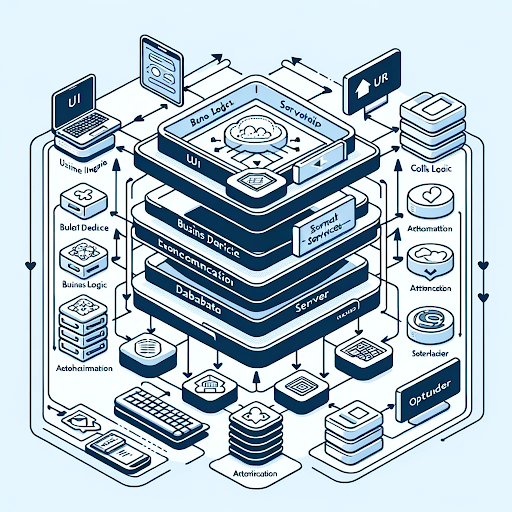
\includegraphics[width=\textwidth]{slike/arhitektura.PNG} %veličina u odnosu na širinu linije
			\centering
			\caption{Osnova arhitekture}
			\label{fig5:promjene}
		\end{figure}
		
		\eject
	
  Skica ilustrira sljedeće komponente i njihovu međusobnu komunikaciju:
   \begin{itemize}
		  \item {Korisničko sučelje (UI): Na klijentskim uređajima (mobitel, tablet, računalo).}
		  \item {Poslovna logika: Dio koji se nalazi na serveru.}	
            \item {Baza podataka: Spremište podataka također na serveru.}
		  \item {Autentikacija: Dio za upravljanje korisničkim pristupom.}	
            \item {Integracija vanjskih usluga: Na primjer, OpenStreetMap za prikaz karata.}
	   \end{itemize}

Izbor Model-View-Controller (MVC) arhitekture za ovu web aplikaciju temelji se na nekoliko ključnih principa oblikovanja koje sam uzimao u obzir:

	\eject
	
	\section{Izbor arhitekture}

 	\subsubsection{Separacija briga (Separation of concerns)}

MVC arhitektura odlično odvaja različite aspekte aplikacije:
\begin{itemize}
		  \item {Model: Predstavlja podatke i poslovnu logiku aplikacije. U ovom slučaju, model bi upravljao podacima knjiga, korisnika, ponuda i zahtjeva za prijevod.}
		  \item {View: Odnosi se na korisničko sučelje. U našoj aplikaciji, ovo bi bilo mjesto gdje korisnici pretražuju knjige, pregledavaju ponude, i komuniciraju sa sustavom.}	
            \item {Controller: Djeluje kao posrednik između Modela i Viewa, obrađuje korisničke zahtjeve, ažurira model i konačno šalje podatke natrag viewu.}
	   \end{itemize}

Ova jasna podjela pomaže u organizaciji koda, olakšava održavanje i omogućava lakše testiranje pojedinih komponenti.
	\\

 \subsubsection{Skalabilnost i fleksibilnost}

MVC podržava skalabilnost. Kako se aplikacija razvija, svaki dio (Model, View, Controller) može se neovisno skalirati ili modificirati. Ovo je posebno korisno za aplikacije koje imaju potencijal rasti, kao što je naš slučaj s web platformom za knjige.
	\\

 \subsubsection{Podrška za više klijentskih platformi}

S obzirom na to da se aplikacija mora prilagoditi različitim uređajima (mobilnim telefonima, tabletima, računalima), MVC omogućava razvoj različitih vrsta viewova koji mogu koristiti isti model i controller logiku. To znači da možemo imati različite korisničke sučelja za mobilne uređaje i desktop računala, dok se poslovna logika i obrada podataka ne mijenjaju.
	\\

 \subsubsection{Održavanje i nadogradnja}

MVC struktura pojednostavljuje ažuriranja i održavanje. Ako trebate promijeniti poslovnu logiku, to se može učiniti u modelu bez utjecaja na view. Slično, izmjene u korisničkom sučelju ne utječu na poslovnu logiku aplikacije.
	\\
	
 \subsubsection{Zajednica i resursi}

MVC je popularan i dobro dokumentiran arhitekturni obrazac. Postoji obilje resursa, biblioteka i okvira koji podržavaju MVC, što može značajno ubrzati razvoj i pružiti bolju podršku tijekom razvojnog procesa.

Zbog ovih razloga, MVC se čini kao optimalan izbor za arhitekturu ove web aplikacije, pružajući dobru osnovu za jasno strukturiran, održiv i fleksibilan razvoj.


Organizacija sustava za opisanu web aplikaciju s najviše razine apstrakcije može se podijeliti u četiri glavne komponente: klijent-poslužitelj model, baza podataka, datotečni sustav, i grafičko sučelje. Ove komponente zajedno omogućavaju funkcionalnost, skalabilnost i korisničku interakciju potrebnu za uspješan rad aplikacije.

	\eject
	
	\section{Organizacija sustava}

 \subsubsection{Klijent-poslužitelj model}

U klijent-poslužitelj modelu, aplikacija je podijeljena na dva glavna dijela: klijent (front-end) koji se izvodi na korisničkom uređaju i poslužitelj (back-end) koji obrađuje zahtjeve i šalje odgovore.
\begin{itemize}
		  \item {Klijent (Front-end): Koristi web preglednik ili mobilnu aplikaciju za pristup aplikaciji. Odgovoran je za prikupljanje korisničkih ulaza, prikazivanje podataka korisnicima i slanje zahtjeva poslužitelju.}
		  \item {Poslužitelj (Back-end): Hostira aplikaciju, obrađuje zahtjeve, vrši operacije nad bazom podataka, i vraća rezultate klijentu. Također upravlja autentikacijom, autorizacijom, i sigurnošću.}	\\
	   \end{itemize}
	   


 \subsubsection{Baza podataka}

Baza podataka je središnje mjesto za pohranu svih podataka koji su relevantni za aplikaciju. Uključuje:
\begin{itemize}
		  \item {Podatke o knjigama: Nazive, autore, žanrove, godine izdanja, itd.}
		  \item {Korisničke podatke: Informacije o registriranim i neregistriranim korisnicima.}	
            \item {Ponude i zahtjeve: Informacije o dostupnosti knjiga, ponuditeljima, i zahtjevima za prijevod.} \\
	   \end{itemize} 


 \subsubsection{Datotečni sustav}

Datotečni sustav se koristi za pohranu i upravljanje datotekama koje nisu direktno povezane s bazom podataka, poput:
\begin{itemize}
		  \item {Slika korica knjiga: Pohranjene kao datoteke koje se mogu prikazivati u korisničkom sučelju.}
		  \item {Dokumenti: Uključujući priručnike, upute za korisnike, i druge dokumente.} \\
	   \end{itemize} 

 \subsubsection{Grafičko sučelje}

Grafičko sučelje (GUI) je ono što korisnik vidi i s čime interagira. Uključuje:
\begin{itemize}
		  \item {Web stranice: Dizajnirane za jednostavno korištenje i navigaciju, s funkcionalnostima kao što su pretraga, pregled knjiga, i slanje zahtjeva.}
		  \item {Mobilno sučelje: Prilagođeno za manje ekrane i osjetljivo na dodir, s sličnim funkcionalnostima kao web verzija.}	\\
	   \end{itemize} 

Svaka od ovih komponenti igra ključnu ulogu u uspješnom funkcioniranju aplikacije, omogućujući efikasnu obradu podataka, intuitivnu korisničku interakciju i sigurnost informacija.

\eject

\section{Organizacija aplikacije}

Organizacija aplikacije koja koristi Model-View-Controller (MVC) arhitekturu s jasno definiranim frontend i backend slojevima omogućava efikasno upravljanje kodom i funkcionalnostima. Evo kako bi se to moglo strukturirati:

 \subsubsection{Frontend (klijentska strana)}

Frontend je ono što korisnik vidi i s čime interagira. U MVC arhitekturi, to uglavnom obuhvaća "View" komponentu.
\begin{itemize}
		  \item {Tehnologije: HTML, CSS, JavaScript, i frameworki poput React, Angular ili Vue.js.}
		  \item {Zadaće:
    \begin{itemize}
		  \item {Prikaz podataka: Dinamički prikazuje podatke dobivene s backend-a.}
		  \item {Korisničko sučelje: Omogućava interakciju s korisnikom, prikuplja korisničke zahtjeve i šalje ih backend-u.}	
            \item {Odgovor na korisničke akcije: Ažuriranje sučelja na temelju korisničkih interakcija i podataka s backend-a.} \\
	   \end{itemize}}	
            
	   \end{itemize}


 \subsubsection{Backend (poslužiteljska strana)}

Backend se bavi obradom podataka, poslovnom logikom i interakcijom s bazom podataka. U MVC arhitekturi, to uključuje "Model" i "Controller" komponente.
\begin{itemize}
		  \item {Tehnologije: Server-side jezici poput Node.js, Python (Django, Flask), Ruby on Rails, Java (Spring), itd.}
		  \item { Zadaće:
            \begin{itemize}
		  \item { Controller:
                    \begin{itemize}
		  \item {Upravlja zahtjevima s frontend-a.}
		  \item {Prosljeđuje podatke između View-a i Modela.}	
            \item {Upravlja tokom podataka i obradi zahtjeva.}
	   \end{itemize}}
        \item { Model:
                    \begin{itemize}
		  \item {Predstavlja poslovnu logiku i podatke.}
		  \item {Interakcija s bazom podataka.}	
            \item {Obrada podataka (CRUD operacije - Create, Read, Update, Delete).} \\
	   \end{itemize}}
	   \end{itemize}}	
	   \end{itemize}


 \subsubsection{Komunikacija između frontend-a i backend-a}

Komunikacija između frontend-a i backend-a obično se odvija preko API-ja (Application Programming Interface), koristeći HTTP/HTTPS protokole.
\begin{itemize}
		  \item {API (najčešće REST ili GraphQL): Definira kako frontend šalje zahtjeve backend-u i kako backend vraća odgovore.}
		  \item {JSON format: Često korišten format za slanje podataka između frontend-a i backend-a.}	\\
	   \end{itemize}


 \subsubsection{Baza podataka}

Iako tehnički nije dio MVC strukture, baza podataka je ključna komponenta koja surađuje s Modelom. Ona pohranjuje sve podatke potrebne za aplikaciju.
\begin{itemize}
		  \item {Tehnologije: SQL (MySQL, PostgreSQL) ili NoSQL (MongoDB, Cassandra) baze podataka.}
		  \item {Zadaće: Pohrana i dohvaćanje podataka potrebnih za aplikaciju.}	
	   \end{itemize}

U ovakvoj organizaciji, svaki sloj ima jasno definiranu ulogu, što doprinosi boljem razumijevanju koda, lakšem održavanju i skaliranju aplikacije. Frontend i backend mogu se neovisno razvijati i optimizirati, što pruža fleksibilnost i efikasnost u razvojnom procesu.

\eject

				
		\section{Baza podataka}
		
		
			\subsection{Opis tablica}
				
				
				\begin{longtblr}[
					label=none,
					entry=none
					]{
						width = \textwidth,
						colspec={|X[8,l]|X[8, l]|X[20, l]|}, 
						rowhead = 1,
					} %definicija širine tablice, širine stupaca, poravnanje i broja redaka naslova tablice
					
					\hline \SetCell[c=3]{c}{\textbf{Korisnik}}	 \\ \hline[3pt]
					\SetCell{LightBlue} & VARCHAR(13) & \\ \hline
					userId & INT & Jedinstveni identifikator, autogeneriran od strane baze \\ \hline
					username & VARCHAR & Jedinstveno korisničko ime \\ \hline
					password & VARCHAR & Jedinstveno lozinka \\ \hline
					naziv & VARCHAR & Naziv korisnika \\ \hline
					adresa & VARCHAR & Adresa korisnika \\ \hline
					telefon & INT & Telefon korisnika \\ \hline
					email & VARCHAR & Email korisnika \\ \hline
					tip & VARCHAR & Tip korisnika \\ \hline
					\\
					
					\hline \SetCell[c=3]{c}{\textbf{Knjiga}}	 \\ \hline[3pt]
					\SetCell{LightGreen} & VARCHAR(13) & \\ \hline
					bookId & INT & Jedinstveni identifikator, autogeneriran od strane baze \\ \hline
					naslov	& VARCHAR & Naziv knjige \\ \hline 
					autor & VARCHAR & Ime autora \\ \hline 
					izdavač & VARCHAR & Ime izdavača	\\ \hline
					brojIzdanja & INT & Broj izdanja knjige	\\ \hline 
					godIzdanja & INT & Godina izdanja knjige	\\ \hline
					kategorija & CHAR(3) & Kategorija izdavača	\\ \hline
					zahtjevi & INT & Zahtjev za prijevod knjige	\\ \hline
					očuvanost & VARCHAR & Očuvanost knjige	\\ \hline
					opis & VARCHAR & Kratki opis knjige	\\ \hline
					slika & VARCHAR & Prikaz knjige	\\ \hline
					žanr & VARCHAR & Žanr knjige \\ \hline
					isbn & INT & ISBN knjige \\ \hline
					\\
					
					\hline \SetCell[c=3]{c}{\textbf{Ponuda}}	 \\ \hline[3pt]
					\SetCell{LightGreen} & VARCHAR(32) & \\ \hline
					offerId	& INT & Jedinstveni identifikator, autogeneriran od strane baze  	\\ \hline 
					nazivPonuditelja & VARCHAR & Naziv ponuditelja  \\ \hline 
					brojPrimjeraka & INT & Broj primjeraka knjige 		\\ \hline 
					cijena & INT & Cijena knjige \\	\hline
					\\
					
			   \end{longtblr}
				
				
			
			\subsection{Dijagram baze podataka} 
				
				\begin{figure}[H]
					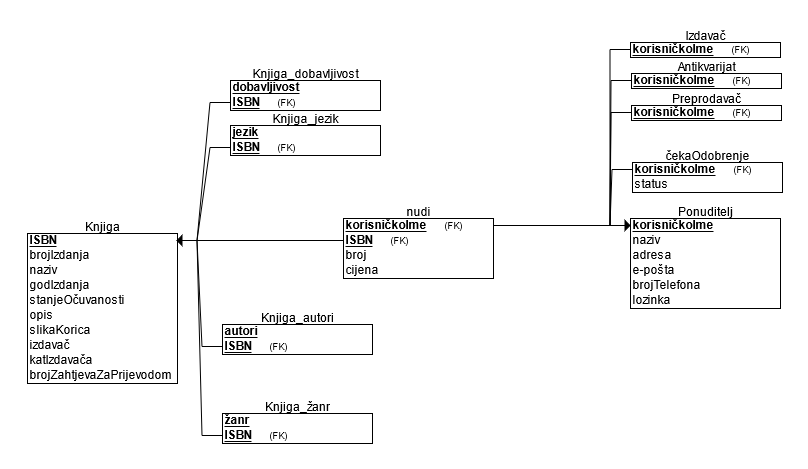
\includegraphics[width=\textwidth]{dijagrami/baza_relmod_v2.PNG} %veličina u odnosu na širinu linije
					\centering
					\caption{REL dijagram baze podataka}
					\label{fig:arh1}
				\end{figure}
				
				\eject
				
				\begin{figure}[H]
					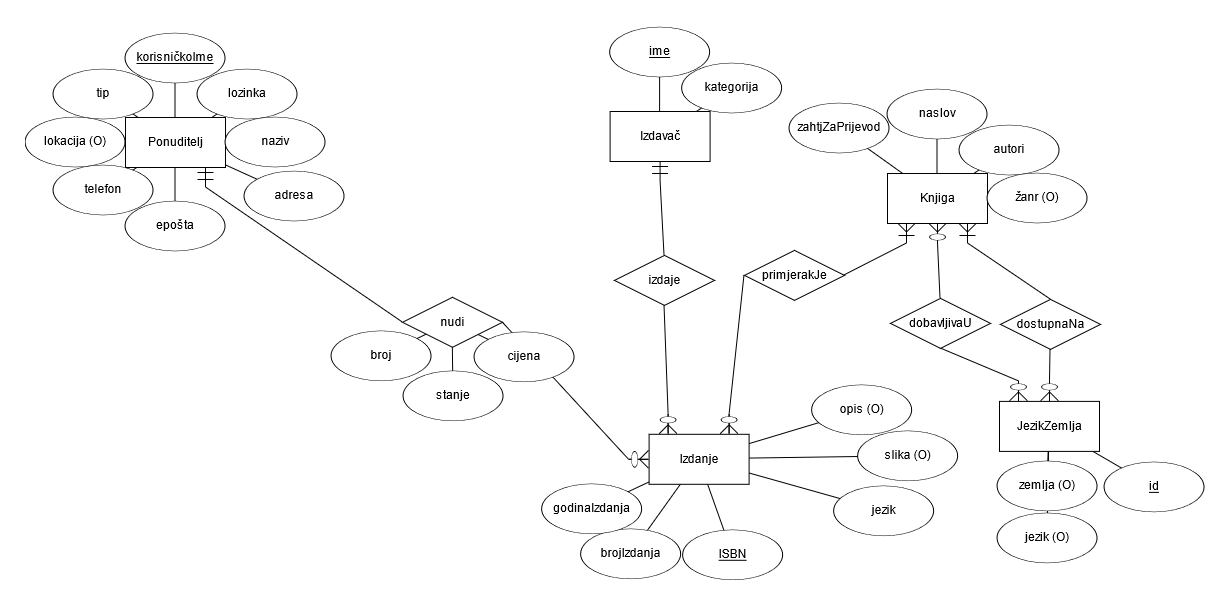
\includegraphics[width=\textwidth]{dijagrami/baza_ERmod_v3.PNG} %veličina u odnosu na širinu linije
					\centering
					\caption{ER dijagram baze podataka}
					\label{fig:arh2}
				\end{figure}
				
			
			\eject
			
			
		\section{Dijagram razreda} 
			
			Idejno razrađeni dijagram razreda opisuje strukturu web aplikacije. Uključuje ApplicationController za upravljanje zahtjevima vezanim uz navigaciju na web stranici, KorisnikController za obrađivanje korisničkih zahtjeva, LoginController za autentikaciju korisnika te Korisnik za predstavljanje entiteta korisnika. KorisnikService brine o logici poslovne logike vezane uz korisnike, dok KorisnikRepository predstavlja sučelje za pristup podacima korisnika u bazi podataka. StoZelisCitatiApplication predstavlja glavni razred aplikacije s main metodom za pokretanje, dok su veze između razreda usmjerene prema ovisnostima i suradnji između njih. Ovo omogućava bolje razumijevanje strukture aplikacije, odvojenost odgovornosti i međusobnu interakciju između komponenti. \\ \\
			
			\begin{figure}[H]
				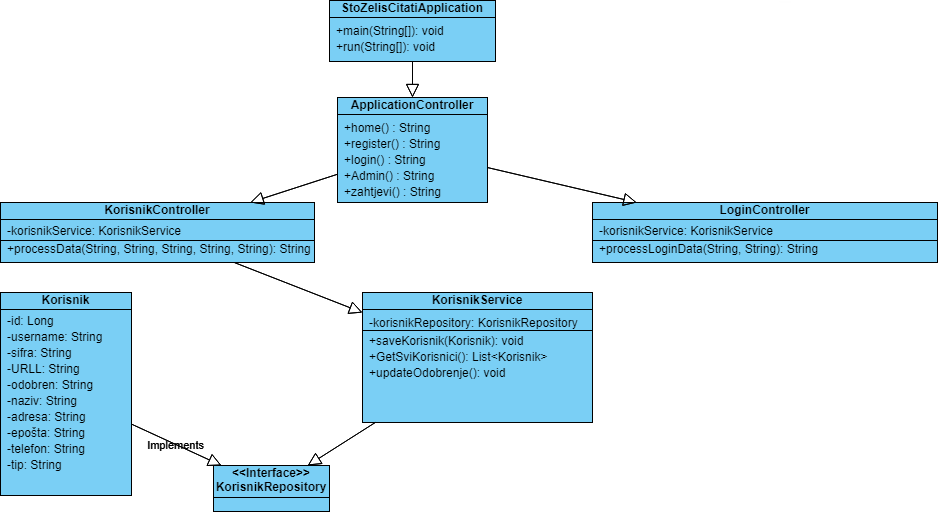
\includegraphics[width=\textwidth]{dijagrami/ClassDiagram1.PNG} %veličina u odnosu na širinu linije
				\centering
				\caption{Dijagram razreda}
				\label{fig:razred}
			\end{figure}
			
			\eject
			
			
			Idejno razrađeni dijagram razreda opisuje sve tri vrste ponuditelja te njihove funkcionalnosti. Predstavljena je ovisnost i suradnja između razreda.
			\\ \\
			
				\begin{figure}[H]
				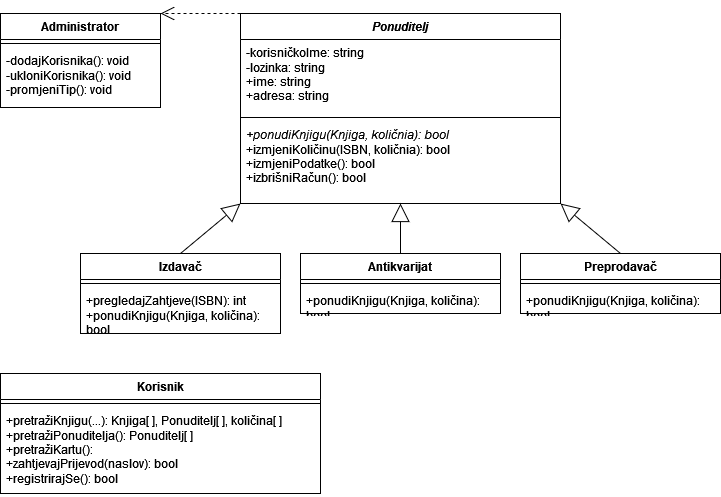
\includegraphics[width=\textwidth]{dijagrami/UML dijagram razreda v1.PNG} %veličina u odnosu na širinu linije
				\centering
				\caption{Dijagram razreda}
				\label{fig:razred1}
			\end{figure}
			
			\eject
			
						
			
			
			\begin{figure}[H]
				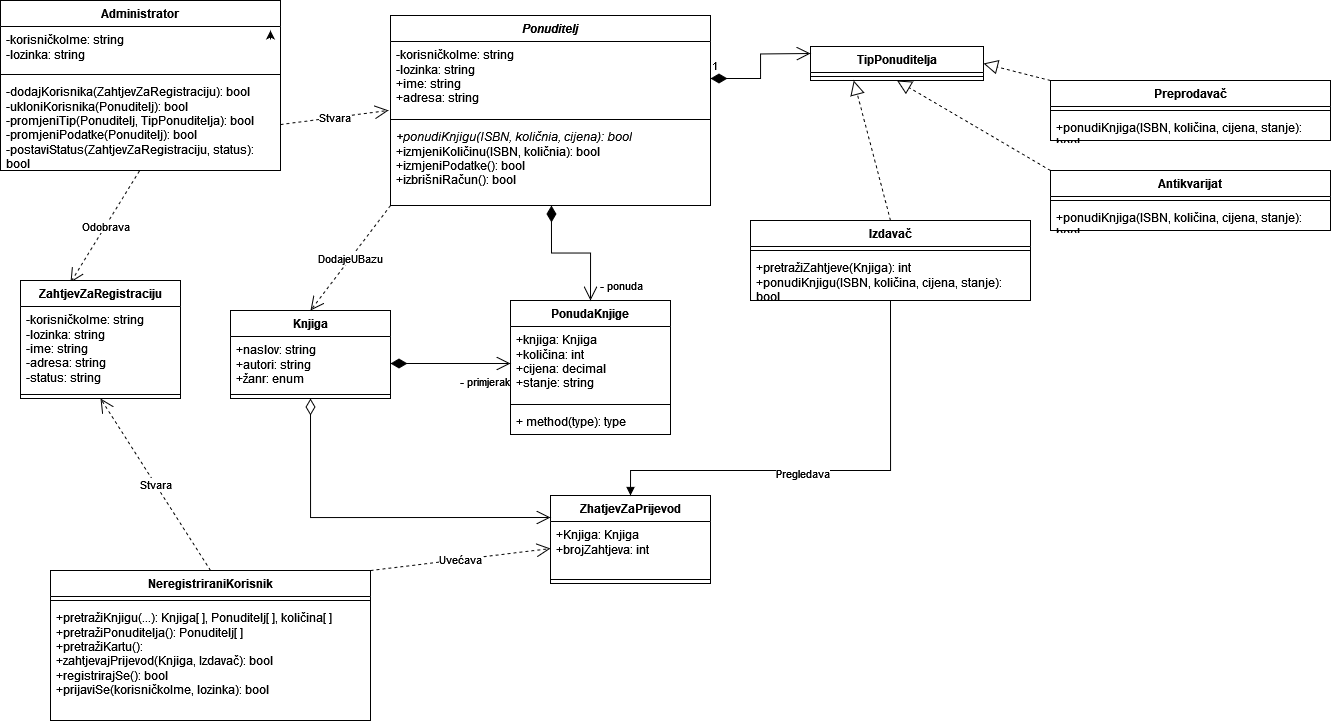
\includegraphics[width=\textwidth]{dijagrami/UML dijagram razreda v2.PNG} %veličina u odnosu na širinu linije
				\centering
				\caption{Dijagram razreda}
				\label{fig:razred2}
			\end{figure}
			
			
			\eject
		
		\section{Dijagram stanja}
			
			
			Dijagram stanja se koristi za modeliranje ponašanja sustava ili entiteta s obzirom na različita stanja kroz koje može proći. Sadrži stanja, prijelaze između stanja, događaje koji pokreću prijelaze te akcije koje se izvršavaju u svakom stanju ili prijelazu. Na slici je prikazan dijagram stanja za registriranog korisnika. Nakon uspješne prijave, korisniku se prikazuje početna stranica na kojoj može vidjeti svoje ponude knjiga te napraviti novu ponudu knjige. Za odabranu knjigu potrebno je provjeriti treba li zatražiti prijevod iste ili ne te zatim unijeti potrebne podatke i zaključiti ponudu. Korisniku se klikom na "Osobni podaci" prikazuju njegovi podaci koje može urediti, a klikom na "Moje ponude" može pregledati sve svoje ponude knjiga.
			
			\eject
			
			
			\begin{figure}[H]
				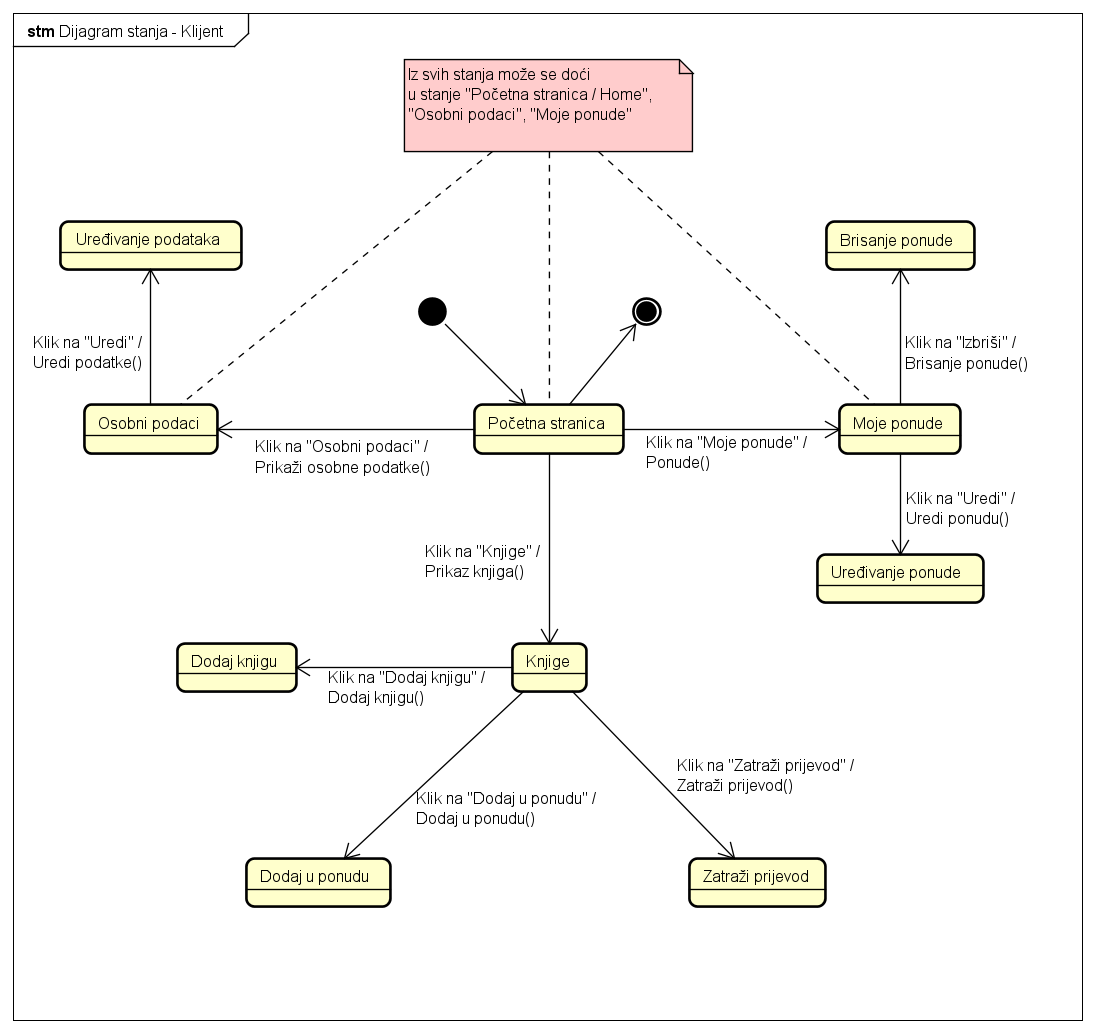
\includegraphics[width=\textwidth]{dijagrami/Dijagram stanja.PNG} %veličina u odnosu na širinu linije
				\centering
				\caption{Dijagram stanja }
				\label{fig:dijagramstanja1}
			\end{figure} 
			
			
			\eject 
		
		\section{Dijagram aktivnosti}
			
			
			Dijagram aktivnosti se koristi za modeliranje poslovnih procesa, algoritama ili drugih sekvenci aktivnosti unutar sustava što je vrlo korisno za opisivanje tokova rada ili procesa izvođenja zadataka. Sadrži stanja, aktivnosti, odluke, ulazne i izlazne tokove te usklađivačke elemente koji pomažu u opisu redoslijeda aktivnosti. Na sljedećem dijagramu prikazan je proces kreiranja nove ponude knjige. Korisnik, nakon prijave u sustav te odobravanja iste, odabire knjigu koju želi dodati u ponudu. Također će zatražiti zahtjev za prijevod ako je to potrebno.
			Nakon unosa svih potrebnih podataka, korisnik zaključuje ponudu. 
			
			\eject
			
			
			\begin{figure}[H]
				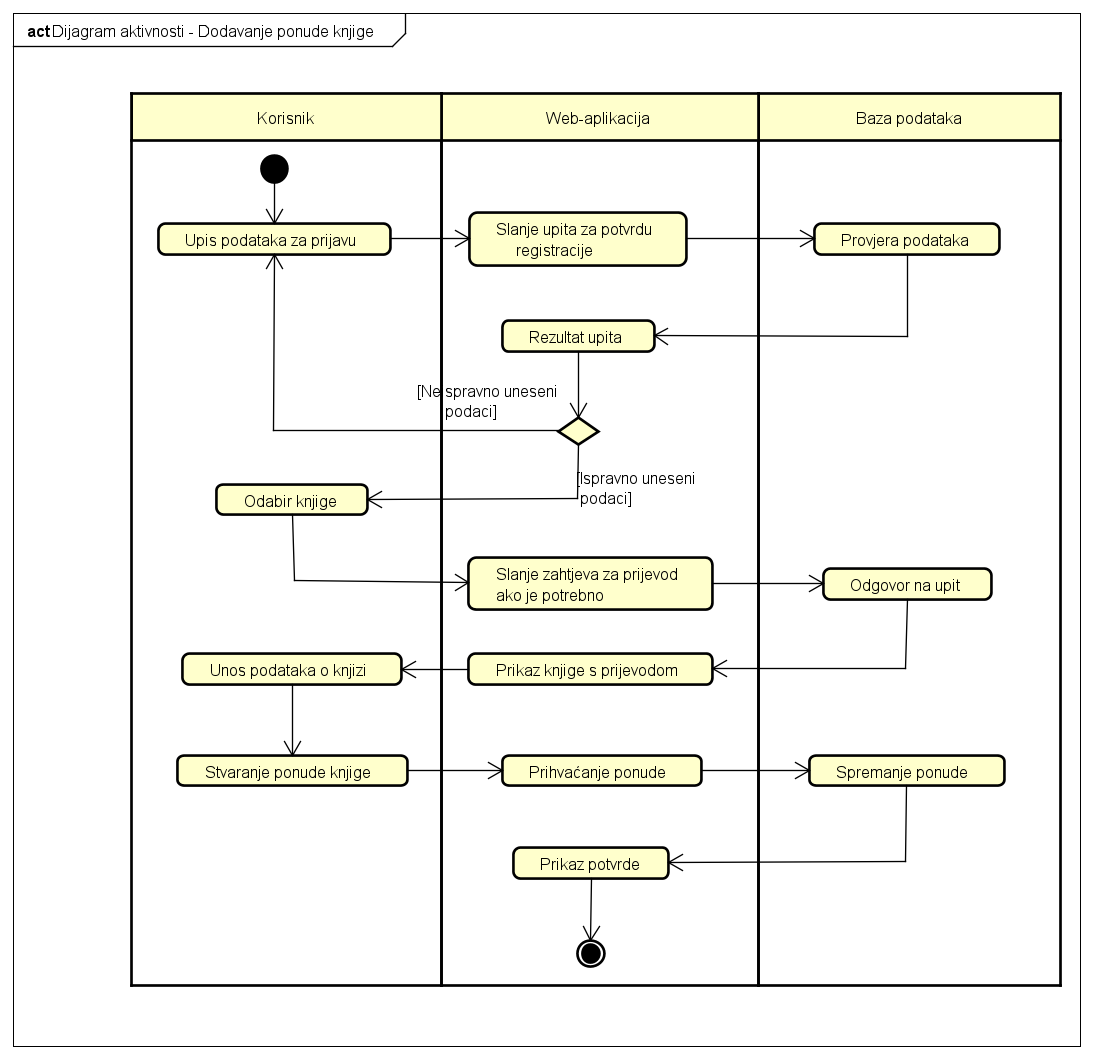
\includegraphics[width=\textwidth]{dijagrami/Dijagram aktivnosti.PNG} %veličina u odnosu na širinu linije
				\centering
				\caption{Dijagram aktivnosti }
				\label{fig:dijagramaktivnosti1}
			\end{figure}
			
			\eject
			
		\section{Dijagram komponenti}
		
			Dijagram komponenti je vrsta strukturnog dijagrama koja prikazuje logičke komponente sustava i njihove odnose. Na ovom dijagramu su vdiljive komponente Prijava, Pretraživanje, Prikaz karte i Prikaz registriranog korisnika koje djeluju unutar React view komponente unutar Frontend web prikaza komponente. One su preko sučelja za dohvat HTML, CSS i JS povezane s komponentom Main.JSX koja funkcionira kao router koji upravlja prikazom i funkcionalnošću grafičkog prikaza. Ovisno o potrebi upravlja ih na komponente AdminPage, RegisterPage, LoginPage, UserPage, BookPage, OfferPage, te HomePage. Sve te komponente se nalaze u Web aplikaciji. Dodatno u Web aplikaciji je komponenta REST API koja je povezana s komponentama za pretraživanje i prikaz registriranog korisnika preko sučelja dohvat JSON. Ona ovisno o potrebi se nadovezuje na Prikaz ponude knjiga koja je preko sučelja SQL povezana s vanjskom komponentom Baza podataka. Ili Prikaz karte koja je preko sučelja REACT API povezana s vanjskom komponento OpenStreetMap. 

            \eject
			
			
			\begin{figure}[H]
				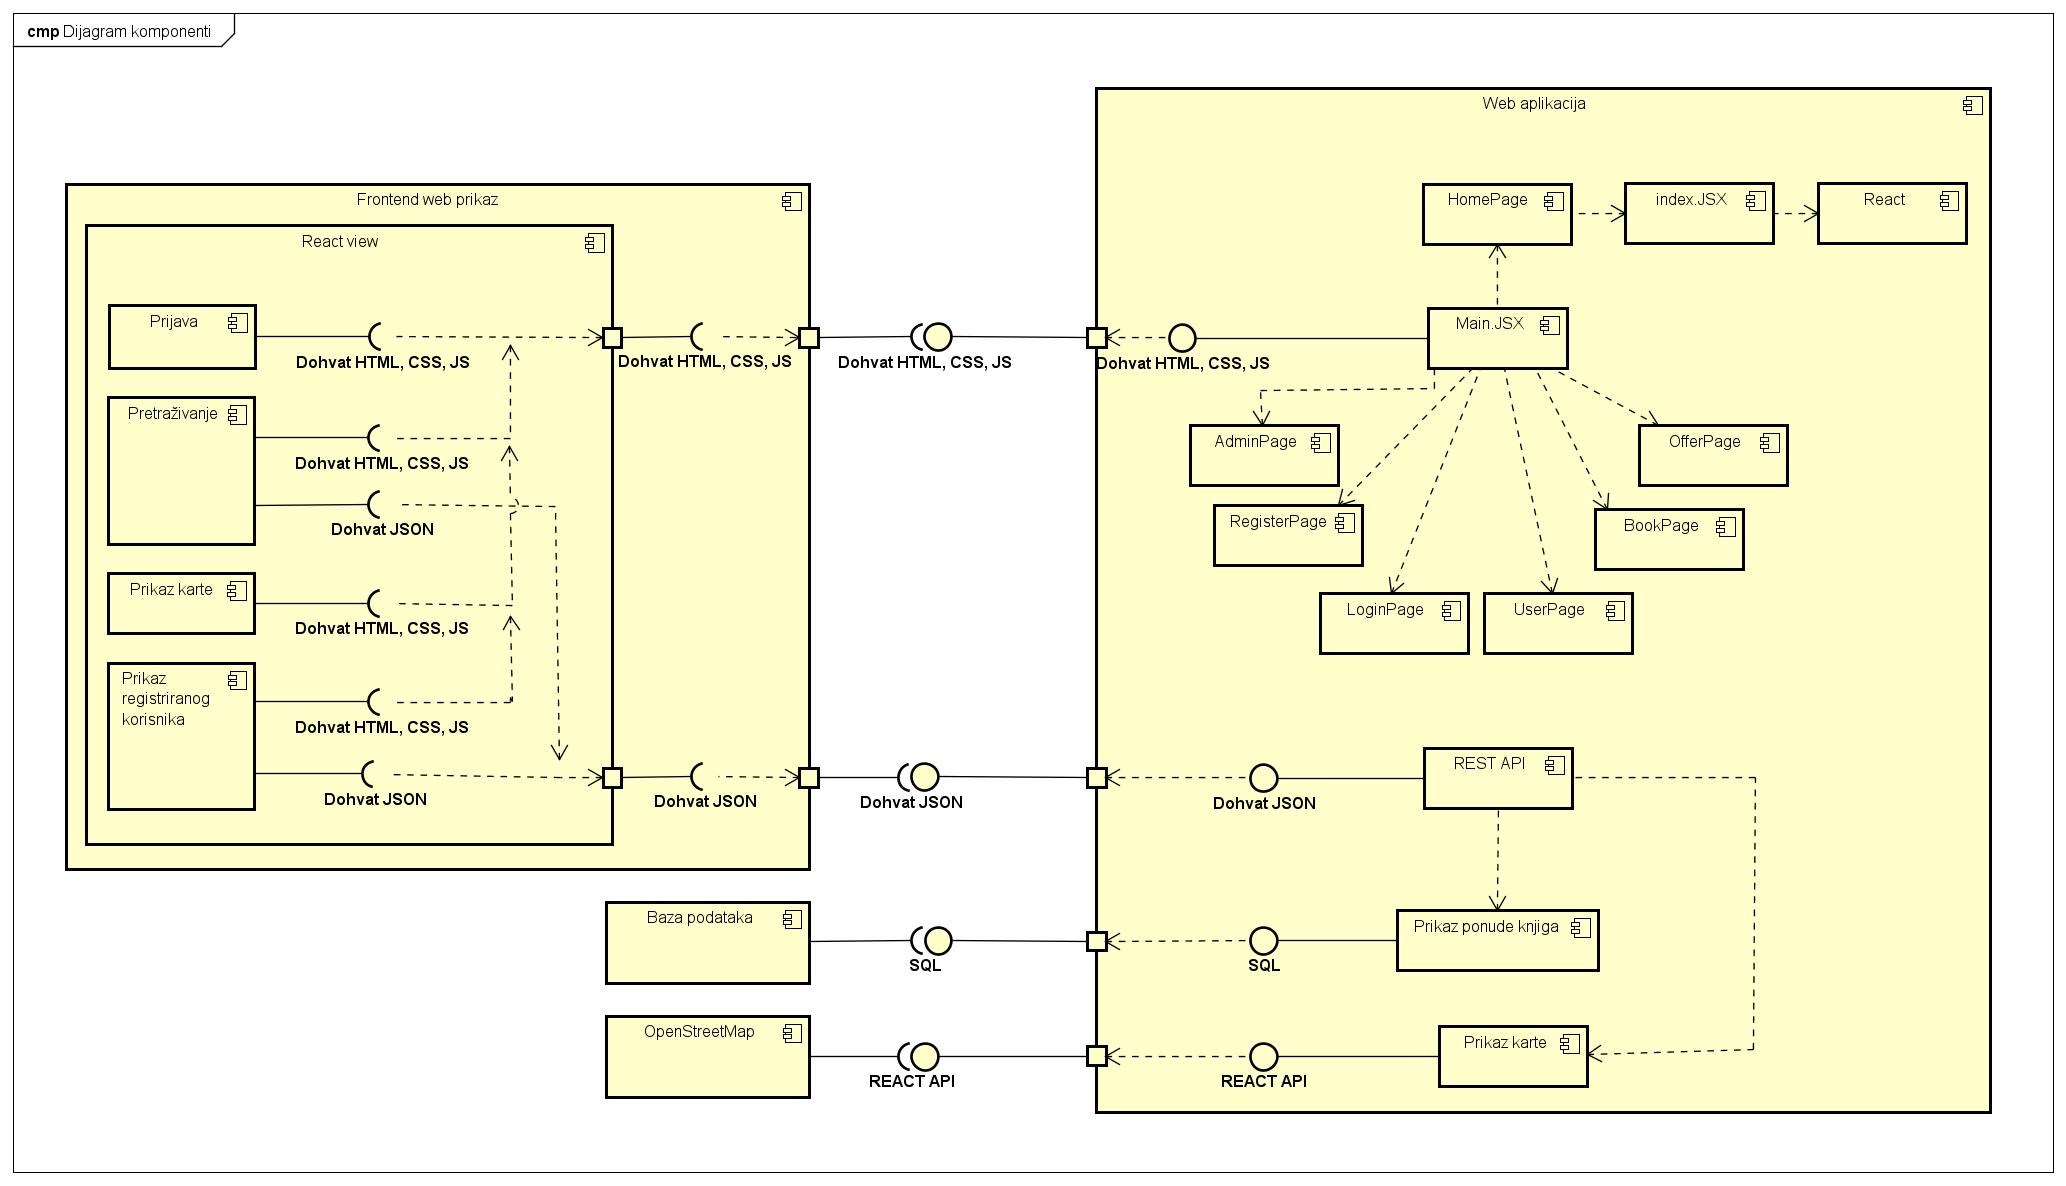
\includegraphics[width=\textwidth]{dijagrami/Dijagram komponenti.PNG} %veličina u odnosu na širinu linije
				\centering
				\caption{Dijagram komponenti }
				\label{fig:dijagramkomponenti1}
			\end{figure}
			
			\eject

	\chapter{Implementacija i korisničko sučelje}
		
		
		\section{Korištene tehnologije i alati}
		
			\textbf{\textit{dio 2. revizije}}
			
			 \textit{Detaljno navesti sve tehnologije i alate koji su primijenjeni pri izradi dokumentacije i aplikacije. Ukratko ih opisati, te navesti njihovo značenje i mjesto primjene. Za svaki navedeni alat i tehnologiju je potrebno \textbf{navesti internet poveznicu} gdje se mogu preuzeti ili više saznati o njima}.
			
			
			\eject 
		
	
		\section{Ispitivanje programskog rješenja}
			
			\textbf{\textit{dio 2. revizije}}\\
			
			 
			
			\subsection{Ispitivanje komponenti}
			     Sastavne programske komponente formirane su od nekoliko jedinica, uključujući osnovne dijelove programa poput razreda, pripadajućih metoda i atributa, koje međusobno intenzivno surađuju. Interakcija se ostvaruje kroz proceduralna sučelja, gdje svaka komponenta enkapsulira određeni skup funkcionalnosti koje druge komponente mogu pozivati. Evaluacija komponenata izvodi se s pomoću Junit radnog okvira, koji automatizira proces testiranja. Upotrebom dviju vrsta testova, jednih u uobičajenim uvjetima rada i drugih s unosom neispravnih i rubnih uvjeta, analizira se očekivano ponašanje razreda i unaprijed definirani izlaz metoda.
            Za testiranje BookService metoda koristili smo sučelja Knjiga, Pondua, i BookRepository. Prvo smo testirali saveBook metodu.
           \begin{lstlisting}[language=Java, label=lst:java_example, basicstyle=\scriptsize, baselinestretch=0.9]
 @Test
    @DisplayName("Testiranje saveBook metode")
    void testSaveBook() {
        // Priprema podataka
        Knjiga knjiga = new Knjiga();
        List<Ponuda> ponude = new ArrayList<>();
        knjiga.setNaziv("Naslov knjige");
        knjiga.setIsbn("100");
        knjiga.setAutor("autor");
        knjiga.setIzdavac("izdavac");
        knjiga.setBrojIzdanja(1);
        knjiga.setOpis("opis");
        knjiga.setGodIzdanja(2005);
        knjiga.setSlikaURL("url");
        knjiga.setId(1L);
        knjiga.setOznaka("oznaka");
        knjiga.setKategorija("kategorija");
        knjiga.setStanjeOcuvanosti("st_oc");
        knjiga.setZahtjevi(50);
        knjiga.setZanr("zanr");
        knjiga.setPonude(ponude);


        when(bookRepository.save(any(Knjiga.class))).thenReturn(knjiga);


        Knjiga savedKnjiga = bookService.saveBook(knjiga);


        verify(bookRepository, times(1)).save(knjiga);
        assertNotNull(savedKnjiga);
        assertEquals("Naslov knjige", savedKnjiga.getNaziv());
        assertEquals("100", savedKnjiga.getIsbn());
        assertEquals("autor", savedKnjiga.getAutor());
        assertEquals("izdavac", savedKnjiga.getIzdavac());
        assertEquals(1, savedKnjiga.getBrojIzdanja());
        assertEquals("opis", savedKnjiga.getOpis());
        assertEquals(2005, savedKnjiga.getGodIzdanja());
        assertEquals("url", savedKnjiga.getSlikaURL());
        assertEquals(1L, savedKnjiga.getId());
        assertEquals("oznaka", savedKnjiga.getOznaka());
        assertEquals("kategorija", savedKnjiga.getKategorija());
        assertEquals("st_oc", savedKnjiga.getStanjeOcuvanosti());
        assertEquals(50, savedKnjiga.getZahtjevi());
        assertEquals("zanr", savedKnjiga.getZanr());
        assertNotNull(savedKnjiga.getPonude());

    }
\end{lstlisting}

   
			A zatim smo testirali deleteBook metodu. 
                  \begin{lstlisting}[language=Java, label=lst:java_example, basicstyle=\scriptsize, baselinestretch=0.9]
 @Test
    @DisplayName("Testiranje deleteBook metode.")
    void testDeleteBook(){
        Long bookIdToDelete = 1L;
        bookService.deleteBook(bookIdToDelete);
        verify(bookRepository).deleteById(bookIdToDelete);
    }
    
\end{lstlisting}

            Zatim smo testirali KorisnikService. Za to smo koristili sučelja Korisnik, Ponuda, i KorisnikRepository.
            
			Prvo smo testirali dohvaćanje korisnika. 
                  \begin{lstlisting}[language=Java, label=lst:java_example, basicstyle=\scriptsize, baselinestretch=0.9]
 @Test
    @DisplayName("Test dohvaćanja korisnika.")
    void testGetUserById() {
        Long userId = 1L;
        Korisnik mockKorisnik = new Korisnik();
        List<Ponuda> ponude = new ArrayList<>();

        mockKorisnik.setId(userId);
        mockKorisnik.setUsername("username");
        mockKorisnik.setPassword("password");
        mockKorisnik.setEmail("email@gmail.com");
        mockKorisnik.setOdobren(false);
        mockKorisnik.setTip("tip");
        mockKorisnik.setAdresa("adresa");
        mockKorisnik.setTelefon("123456789");
        mockKorisnik.setPonude(ponude);
        mockKorisnik.setPrijavljen(false);
        mockKorisnik.setURLL("url");
        mockKorisnik.setNaziv("naziv");

        when(korisnikRepository.findById(userId)).thenReturn(Optional.of(mockKorisnik));

        Korisnik result = korisnikService.getUserById(userId);

        assertEquals(userId, result.getId());
        assertEquals("adresa", result.getAdresa());
        assertEquals("123456789", result.getTelefon());
        assertEquals("tip", result.getTip());
        assertEquals("email@gmail.com", result.getEmail());
        assertEquals("password", result.getPassword());
        assertEquals("username", result.getUsername());
        assertEquals(false, result.getOdobren());
        assertNotNull(ponude);
        assertEquals(false, result.isPrijavljen());
        assertEquals("url", result.getURLL());
        assertEquals("naziv", result.getNaziv());
    }

    
\end{lstlisting}
            
			Zatim smo testirali funkcionalnost spremanja korisnika. 
                  \begin{lstlisting}[language=Java, label=lst:java_example, basicstyle=\scriptsize, baselinestretch=0.9]
 @Test
    @DisplayName("Test spremanja korisnika.")
    void saveUserTest(){
        Long userId = 1L;
        Korisnik mockKorisnik = new Korisnik();
        List<Ponuda> ponude = new ArrayList<>();

        mockKorisnik.setId(userId);
        mockKorisnik.setUsername("username");
        mockKorisnik.setPassword("password");
        mockKorisnik.setEmail("email@gmail.com");
        mockKorisnik.setOdobren(false);
        mockKorisnik.setTip("tip");
        mockKorisnik.setAdresa("adresa");
        mockKorisnik.setTelefon("123456789");
        mockKorisnik.setPonude(ponude);
        mockKorisnik.setPrijavljen(false);
        mockKorisnik.setURLL("url");
        mockKorisnik.setNaziv("naziv");


        when(korisnikRepository.save(any(Korisnik.class))).thenReturn(mockKorisnik);

        Korisnik savedKorisnik = korisnikService.saveKorisnik(mockKorisnik);

        verify(korisnikRepository, times(1)).save(mockKorisnik);
        
        assertEquals(userId, savedKorisnik.getId());
        assertEquals("adresa", savedKorisnik.getAdresa());
        assertEquals("123456789", savedKorisnik.getTelefon());
        assertEquals("tip", savedKorisnik.getTip());
        assertEquals("email@gmail.com", savedKorisnik.getEmail());
        assertEquals("password", savedKorisnik.getPassword());
        assertEquals("username", savedKorisnik.getUsername());
        assertEquals(false, savedKorisnik.getOdobren());
        assertNotNull(ponude);
        assertEquals(false, savedKorisnik.isPrijavljen());
        assertEquals("url", savedKorisnik.getURLL());
        assertEquals("naziv", savedKorisnik.getNaziv());
    }
    
\end{lstlisting}
            
			Nakon toga smo testirali ponudu, to jest OfferService. Za te testove smo koristili sučelja Knjiga, Korisnik, Ponuda, PonudaDto, BookRepository, KorisnikRepository, OfferRepository i OfferService. 
            Prvo smo testirali brisanje ponude. 
            
                  \begin{lstlisting}[language=Java, label=lst:java_example, basicstyle=\scriptsize, baselinestretch=0.9]
 @Test
    @DisplayName("Testiranje brisanja ponude.")
    void deleteOfferTest() {
        Long offerId = 1L;

        offerService.deleteOffer(offerId);

        verify(offerRepository, times(1)).deleteById(offerId);
    }
    
\end{lstlisting}
            A zatim smo testirali spremanje ponude. 
                  \begin{lstlisting}[language=Java, label=lst:java_example, basicstyle=\scriptsize, baselinestretch=0.9]
  @Test
    @DisplayName("Testiranje spremanja ponude.")
    void saveOffer() {
        // Arrange
        PonudaDto ponudaDto = new PonudaDto();
        ponudaDto.setPonuditeljId(1L);
        ponudaDto.setKnjigaId(2L);
        ponudaDto.setCijena(100);
        ponudaDto.setBrojPrimjeraka(5);

        Korisnik mockKorisnik = new Korisnik();
        Knjiga mockKnjiga = new Knjiga();
        Ponuda mockPonuda = new Ponuda();

        when(korisnikRepository.findById(ponudaDto.getPonuditeljId())).thenReturn(java.util.Optional.of(mockKorisnik));
        when(bookRepository.findById(ponudaDto.getKnjigaId())).thenReturn(java.util.Optional.of(mockKnjiga));
        when(offerRepository.save(any(Ponuda.class))).thenReturn(mockPonuda);


        Ponuda resultPonuda = offerService.saveOffer(ponudaDto);

        verify(offerRepository).save(any(Ponuda.class));

        assertEquals(mockPonuda, resultPonuda);
    }

    
\end{lstlisting}
            Zatim smo testirali kada spremamo ponudu, a ne postoji taj userId.
                  \begin{lstlisting}[language=Java, label=lst:java_example, basicstyle=\scriptsize, baselinestretch=0.9]
 @Test
    @DisplayName("Testiranje kada spremamo ponudu. a ne postoji taj userId.")
    void saveOfferInvalid() {
        PonudaDto ponudaDto = new PonudaDto();
        ponudaDto.setPonuditeljId(1L);
        ponudaDto.setKnjigaId(2L);
        ponudaDto.setCijena(100);
        ponudaDto.setBrojPrimjeraka(5);

        when(korisnikRepository.findById(ponudaDto.getPonuditeljId())).thenReturn(Optional.empty());

        // Act & Assert
        // Verify that ResponseStatusException is thrown with the correct status and message
        ResponseStatusException exception = Assertions.assertThrows(ResponseStatusException.class, () -> {
            offerService.saveOffer(ponudaDto);
        });

        assertEquals(HttpStatus.NOT_FOUND, exception.getStatusCode());
        assertEquals("Korisnik not found", exception.getReason());
    }
    
\end{lstlisting}

            Svi testovi su se ispravno izveli s očekivanim rezultatima. 
            \eject
			
			
			\begin{figure}[H]
				\includegraphics[width=\textwidth]{slike/UnitiTest1.PNG} %veličina u odnosu na širinu linije
				\centering
				\caption{Rezultat testiranja BookService }
				\label{fig:BookService1}
			\end{figure}
			
			\eject
            \eject
			
			
			\begin{figure}[H]
				\includegraphics[width=\textwidth]{slike/UnitiTest3.PNG} %veličina u odnosu na širinu linije
				\centering
				\caption{Rezultat testiranja KorisnikService }
				\label{fig:KorisnikService1}
			\end{figure}
			
			\eject
            \eject
			
			
			\begin{figure}[H]
				\includegraphics[width=\textwidth]{slike/UnitiTest3.PNG} %veličina u odnosu na širinu linije
				\centering
				\caption{Rezultat testiranja OfferService}
				\label{fig:OfferService1}
			\end{figure}
			
			\eject
			
			
			
			
			
			\subsection{Ispitivanje sustava}
			
			 \textit{Potrebno je provesti i opisati ispitivanje sustava koristeći radni okvir Selenium\footnote{\url{https://www.seleniumhq.org/}}. Razraditi \textbf{minimalno 4 ispitna slučaja} u kojima će se ispitati redovni slučajevi, rubni uvjeti te poziv funkcionalnosti koja nije implementirana/izaziva pogrešku kako bi se vidjelo na koji način sustav reagira kada nešto nije u potpunosti ostvareno. Ispitni slučaj se treba sastojati od ulaza (npr. korisničko ime i lozinka), očekivanog izlaza ili rezultata, koraka ispitivanja i dobivenog izlaza ili rezultata.\\ }
			 
			 \textit{Izradu ispitnih slučajeva pomoću radnog okvira Selenium moguće je provesti pomoću jednog od sljedeća dva alata:}
			 \begin{itemize}
			 	\item \textit{dodatak za preglednik \textbf{Selenium IDE} - snimanje korisnikovih akcija radi automatskog ponavljanja ispita	}
			 	\item \textit{\textbf{Selenium WebDriver} - podrška za pisanje ispita u jezicima Java, C\#, PHP koristeći posebno programsko sučelje.}
			 \end{itemize}
		 	\textit{Detalji o korištenju alata Selenium bit će prikazani na posebnom predavanju tijekom semestra.}
			
			\eject 
		
		
		\section{Dijagram razmještaja}
			
			Dijagrami razmještaja prikazuju fizičku arhitekturu i topologiju programskog sustava te programsku potporu koja se koristi u njegovom radnom okruženju. Na korisničkom računalu se nalazi web preglednik koji služi za pristupanje web aplikaciji. Na poslužiteljskom računalu se nalaze web poslužitelj i poslužitelj baze podataka koji međusobno komuniciraju. Sustav koristi arhitekturu "klijent - poslužitelj", a komunikacija između korisnika(klijent, izdavač, administrator) i poslužitelja se odvija preko HTTP protokola.
			
			\begin{figure}[H]
				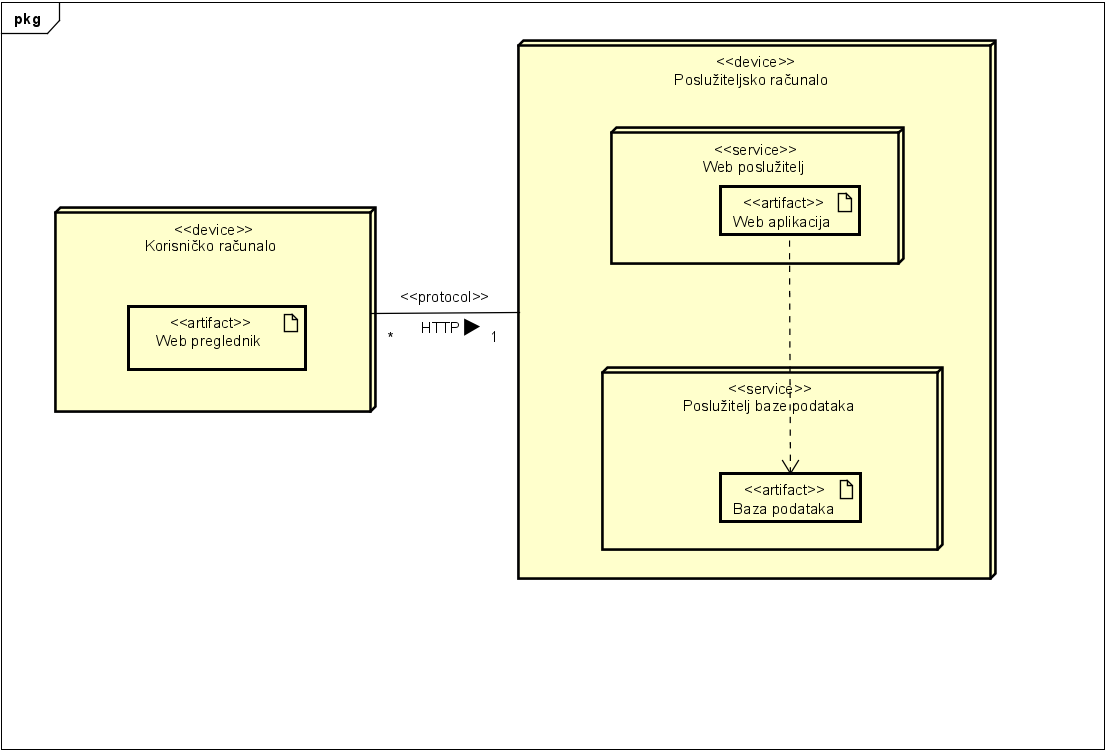
\includegraphics[width=\textwidth]{dijagrami/DijagramRazmjestaja.PNG} %veličina u odnosu na širinu linije
				\centering
				\caption{Dijagram razmještaja}
				\label{fig:diagrazmjestaja}
			\end{figure}
			
			
			\eject 
		
		\section{Upute za puštanje u pogon}
		
			\textbf{\textit{dio 2. revizije}}\\
		
			 \textit{U ovom poglavlju potrebno je dati upute za puštanje u pogon (engl. deployment) ostvarene aplikacije. Na primjer, za web aplikacije, opisati postupak kojim se od izvornog kôda dolazi do potpuno postavljene baze podataka i poslužitelja koji odgovara na upite korisnika. Za mobilnu aplikaciju, postupak kojim se aplikacija izgradi, te postavi na neku od trgovina. Za stolnu (engl. desktop) aplikaciju, postupak kojim se aplikacija instalira na računalo. Ukoliko mobilne i stolne aplikacije komuniciraju s poslužiteljem i/ili bazom podataka, opisati i postupak njihovog postavljanja. Pri izradi uputa preporučuje se \textbf{naglasiti korake instalacije uporabom natuknica} te koristiti što je više moguće \textbf{slike ekrana} (engl. screenshots) kako bi upute bile jasne i jednostavne za slijediti.}
			
			
			 \textit{Dovršenu aplikaciju potrebno je pokrenuti na javno dostupnom poslužitelju. Studentima se preporuča korištenje neke od sljedećih besplatnih usluga: \href{https://aws.amazon.com/}{Amazon AWS}, \href{https://azure.microsoft.com/en-us/}{Microsoft Azure} ili \href{https://www.heroku.com/}{Heroku}. Mobilne aplikacije trebaju biti objavljene na F-Droid, Google Play ili Amazon App trgovini.}
			
			
			\eject 

	\chapter{Zaključak i budući rad}
		
		\textbf{\textit{dio 2. revizije}}\\
		
		 \textit{Naša grupa za projektni zadatak je dobila izradu i razvoj web aplikacije pod nazivom: „Što želiš čitati?“  koja omogućuje čitateljima pretragu ponuditelja knjiga na mapi, te pretragu knjiga na temelju njihove dostupnosti na hrvatskom jeziku i tržištu, također im i omogućavam zahtjev za prijevod knjige ako on već ne postoji. S druge strane ponuditeljima knjiga, izdavačima, antikvarijatima i preprodavačima omogućava ponudu knjiga većoj publici i tako poboljšanje poslovanja. Kroz četrnaest tjedana timskog rada uspješno smo ostvarili cilj i uz to smo stekli nova znanja i vještine. Projekt se razvijao u dvije faze. }
		
		 \textit{Prva faza je započela okupljanjem tima, dijeljenjem ideja o razvoju projekta, određivanju ciljeva, te izražavanju pojedinačnih interesa i kompetencija na području razvoja web aplikacije, te razvoja samog projekta. Uzevši sve u obzir raspodijelili smo potrebni posao po mogućnostima i željama svakoga člana, te smo odredili rokove predaje. Podijelili smo se u dva tima, prvi od četiri člana zadužen za dokumentaciju i drugi od tri člana zaduženi za početnu implementaciju. Prva faza je trajala do kolokvija uz malo kašnjenje pri predaji.}
   
          \textit{Nakon što smo dobili ocjenu prve faze i pomoćne savijete što popraviti i kako se poboljšati u drugoj fazi, sastali smo se, raspravili smo o tome što je dobro bilo u prvoj fazi, a što je pošlo po zlu i uzrokovalo kašnjenje, te što možemo učiniti u drugoj fazi da to izbjegnemo. Zaključili smo da bi nam češći sastanci, i raspodjela zadataka na manje komponente s češćim rokovima predaje pomogla da uspješno i na vrijeme odradimo vlastite zadatke. I to bi nam omogućilo praćenje ako tko ima kakvih problema sa svojim zadatkom i brzu intervenciju, kako bi izbjegli veće zaostatke u razvoju.  Budući da smo se svi planirali baviti implementacijom u drugoj fazi, tim za implementaciju iz prve faze nam je predstavio što su oni bili implementirali i predložio kako da se raspodijelimo. Međusobno smo raspodijelili pravljenje potrebne dokumentacije, te smo ju napravili na početku druge faze kako bi se mogli nesmetano prebaciti na implementaciju.  S time smo bili uglavnom uspješni uz nedostatak par funkcionalnosti poput provjere adresa registriranih korisnika. To jest ne ograničavamo registrirane korisnike na područje djelovanja njihove vrste kako je specijalizirano u zadatku. Također omogućili smo da sve knjige imaju mogućnost zahtjeva za prijevod, a ne samo one na stranom jeziku.  Te kod registracije ne provjeravamo je li željena e-mail adresa ili ime već zauzeto.}
          
          \textit{Sve u svemu sudjelovanje u ovom projektu je vrijedno iskustvo za svakoga člana, osim što smo naučili kako funkcionira izrada web aplikacije, kako se koristiti JavaScript bibliotekom react, i okvir za razvoj Java aplikacija Spring, te ostale tehnologije, naučili smo kako je to raditi u timu.  Spoznali smo važnost dobre komunikacije i kako dobro postavljeni rokovi i dobro definirani zadatci olakšavaju izvođenje projekta. Svjesni smo da ima prostora za poboljšanje, ali zadovoljni smo postignutim uspjehom i znanjima koje smo stekli, te se veselimo budućem radu i potencijalnoj suradnji.}
		
		\eject 

	\chapter*{Popis literature}
		\addcontentsline{toc}{chapter}{Popis literature}
		
		
		\begin{enumerate}
			
			
			\item  Programsko inženjerstvo, FER ZEMRIS, \url{http://www.fer.hr/predmet/proinz}
			
			\item  I. Sommerville, "Software engineering", 8th ed, Addison Wesley, 2007.
			
			\item  T.C.Lethbridge, R.Langaniere, "Object-Oriented Software Engineering", 2nd ed. McGraw-Hill, 2005.
			
			\item  I. Marsic, Software engineering book``, Department of Electrical and Computer Engineering, Rutgers University, \url{http://www.ece.rutgers.edu/~marsic/books/SE}
			
			\item  The Unified Modeling Language, \url{https://www.uml-diagrams.org/}
			
			\item  Astah Community, \url{http://astah.net/editions/uml-new}
			
			\item Junit5, \url{https://junit.org/junit5/}
			
		\end{enumerate}
		
		 
	
	
	\begingroup
	\renewcommand*\listfigurename{Indeks slika i dijagrama}
	%\renewcommand*\listtablename{Indeks tablica}
	%\let\clearpage\relax
	\listoffigures
	%\vspace{10mm}
	%\listoftables
	\endgroup
	\addcontentsline{toc}{chapter}{Indeks slika i dijagrama}


	
	\eject 
		
	\chapter*{Dodatak: Prikaz aktivnosti grupe}
		\addcontentsline{toc}{chapter}{Dodatak: Prikaz aktivnosti grupe}
		
		\section*{Dnevnik sastajanja}
	
		
		\begin{packed_enum}
			\item  sastanak
			
			\item[] \begin{packed_item}
				\item Datum: 21. listopada 2023.
				\item Prisustvovali: R. Balun, L. Blagaić, A. Gazibarić, D. Marenić, F. Šturlić, Š. Vuletić, L. Zelić
				\item Teme sastanka:
				\begin{packed_item}
					\item  upoznavanje s zadatkom
					\item  odabir baznih tehnologija
					\item  proučavanje dokumentacije i podjela poslova
				\end{packed_item}
			\end{packed_item}
			
			\item  sastanak
			\item[] \begin{packed_item}
				\item Datum: 5. studenoga 2023.
				\item Prisustvovali: R. Balun, L. Blagaić, A. Gazibarić, D. Marenić, F. Šturlić, Š. Vuletić, L. Zelić
				\item Teme sastanka:
				\begin{packed_item}
					\item  dodatni dogovor oko raspodjele zadataka
					\item  proučavanje implementacije i podjela poslova
					\item  dogovor oko korištenih tehnologija za implementaciju
				\end{packed_item}
			\end{packed_item}
			
			\item  sastanak
			\item[] \begin{packed_item}
				\item Datum: 12. studenoga 2023.
				\item Prisustvovali: R. Balun, L. Blagaić, A. Gazibarić, D. Marenić, F. Šturlić, Š. Vuletić, L. Zelić
				\item Teme sastanka:
				\begin{packed_item}
					\item  provjera valjanosti dokumentacije
					\item  provjera valjanosti implementacije
					\item  dogovor oko puštanja aplikacije u pogon
				\end{packed_item}
			\end{packed_item}
			
			\item  sastanak
			\item[] \begin{packed_item}
				\item Datum: 26. prosinca 2023.
				\item Prisustvovali: R. Balun, L. Blagaić, A. Gazibarić, D. Marenić, F. Šturlić, Š. Vuletić, L. Zelić
				\item Teme sastanka:
				\begin{packed_item}
					\item  dogovor oko budućeg rada
					\item  predložene promjene oko izrade aplikacije
					\item  raspodjela zadataka vezanih za dokumentaciju
				\end{packed_item}
			\end{packed_item}
			
			\item  sastanak
			\item[] \begin{packed_item}
				\item Datum: 30. prosinca 2023.
				\item Prisustvovali: R. Balun, L. Blagaić, A. Gazibarić, D. Marenić, F. Šturlić, Š. Vuletić, L. Zelić
				\item Teme sastanka:
				\begin{packed_item}
					\item  detaljan opis implementacije i korištenih tehnologija
					\item  raspodjela zadataka vezanih za implementaciju
				\end{packed_item}
			\end{packed_item}
			
			\item  sastanak
			\item[] \begin{packed_item}
				\item Datum: 8. siječnja 2024.
				\item Prisustvovali: A. Gazibarić, D. Marenić, F. Šturlić, Š. Vuletić, L. Zelić
				\item Teme sastanka:
				\begin{packed_item}
					\item  zajedničko implementiranje zadataka
					\item  dogovor oko sljedećih zadataka
					\item  raspodjela poslova
				\end{packed_item}
			\end{packed_item}
			
			\item  sastanak
			\item[] \begin{packed_item}
				\item Datum: 17. siječnja 2024.
				\item Prisustvovali: R. Balun, L. Blagaić, A. Gazibarić, F. Šturlić, Š. Vuletić, L. Zelić
				\item Teme sastanka:
				\begin{packed_item}
					\item  dovršavanje zasebnih zadataka implementacije
					\item  dogovor oko puštanja aplikacije u pogon
				\end{packed_item}
			\end{packed_item}
			
			%
			
		\end{packed_enum}
		
		\eject
		\section*{Tablica aktivnosti}
		

			\begin{longtblr}[
					label=none,
				]{
					vlines,hlines,
					width = \textwidth,
					colspec={X[7, l]X[1, c]X[1, c]X[1, c]X[1, c]X[1, c]X[1, c]X[1, c]}, 
					vline{1} = {1}{text=\clap{}},
					hline{1} = {1}{text=\clap{}},
					rowhead = 1,
				} 
			
				\SetCell[c=1]{c}{} & \SetCell[c=1]{c}{\rotatebox{90}{\textbf{Andrea Gazibarić}}} & \SetCell[c=1]{c}{\rotatebox{90}{\textbf{Renato Balun }}} &	\SetCell[c=1]{c}{\rotatebox{90}{\textbf{Luka Blagaić }}} & \SetCell[c=1]{c}{\rotatebox{90}{\textbf{Davor Marenić }}} &	\SetCell[c=1]{c}{\rotatebox{90}{\textbf{Filip Šturlić }}} & \SetCell[c=1]{c}{\rotatebox{90}{\textbf{Šima Vuletić }}} &	\SetCell[c=1]{c}{\rotatebox{90}{\textbf{Luka Zelić }}} \\   
				Opis projektnog zadatka 	&  &  &  &  &  &2  & \\ 
				
				Funkcionalni zahtjevi       &  &  &2  &  &  &  &  \\ 
				Opis pojedinih obrazaca 	&3  &  &  &  &  &  &  \\ 
				Dijagram obrazaca 			&2  &  &  &  &  &  &  \\ 
				Sekvencijski dijagrami 		&  &2  &  &  &  &  &  \\ 
				Opis ostalih zahtjeva 		&  &  &  &  &  &  &1  \\ 

				Arhitektura i dizajn sustava	 &  &  &  &2  &  &  &  \\ 
				Baza podataka				&  &  &3  &  &  &  &   \\ 
				Dijagram razreda 			&  &  &2  &  &  &  &   \\ 
				Dijagram stanja				&2  &  &  &  &  &  &  \\ 
				Dijagram aktivnosti 		&2  &  &  &  &  &  &  \\ 
				Dijagram komponenti			&  &  &  &  &  &2  &  \\ 
				Korištene tehnologije i alati 		&  &  &2  &  &  &  &  \\ 
				Ispitivanje programskog rješenja 	&  &3  &  &  &  &3  &  \\ 
				Dijagram razmještaja			&  &2  &  &  &  &  &  \\ 
				Upute za puštanje u pogon 		&  &  &  &  &  &  &1  \\  
				Dnevnik sastajanja 			&1  &  &  &  &  &  &  \\ 
				Zaključak i budući rad 		&  &  &  &  &  &2  &  \\  
				Popis literature 			&  &  &  &  &  &1  &  \\  
				\\
				back end 			&40  &5  &5  &2  &2  &2  &35  \\ 
				front end 			&40  &5  &5  &2  &5  &5  &35  \\  
				izrada baze podataka 		&  &  &5  &  &  &  & \\  
				deployment 	 				&4  &  &  &  &  &  &10  \\ 
				izrada dijagrama			&5  &5  &5  &  &5  &5  &  \\  
				istraživanje 				&5  &5  &5  &5  &5  &5  &5\\ 
			\end{longtblr}
					
					
		\eject
		\section*{Dijagrami pregleda promjena}
		
		\begin{figure}[H]
			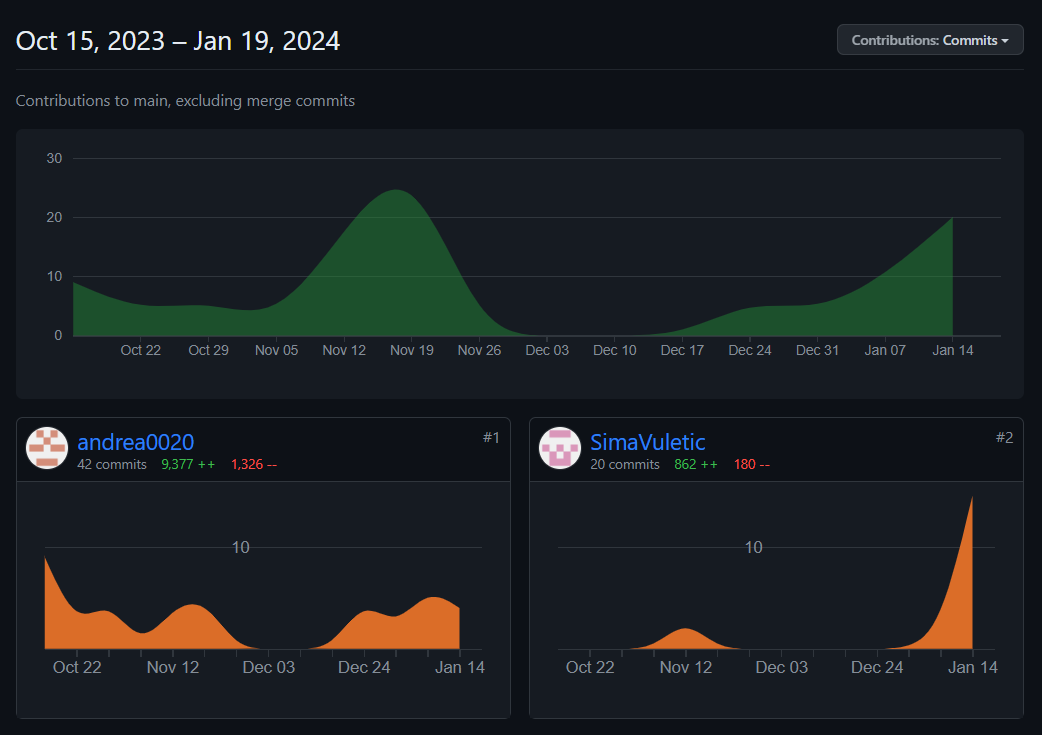
\includegraphics[width=\textwidth]{slike/d1.PNG} %veličina u odnosu na širinu linije
			\centering
			\caption{Graf GitHub aktivnosti}
			\label{fig:d1}
		\end{figure}
		
		\begin{figure}[H]
			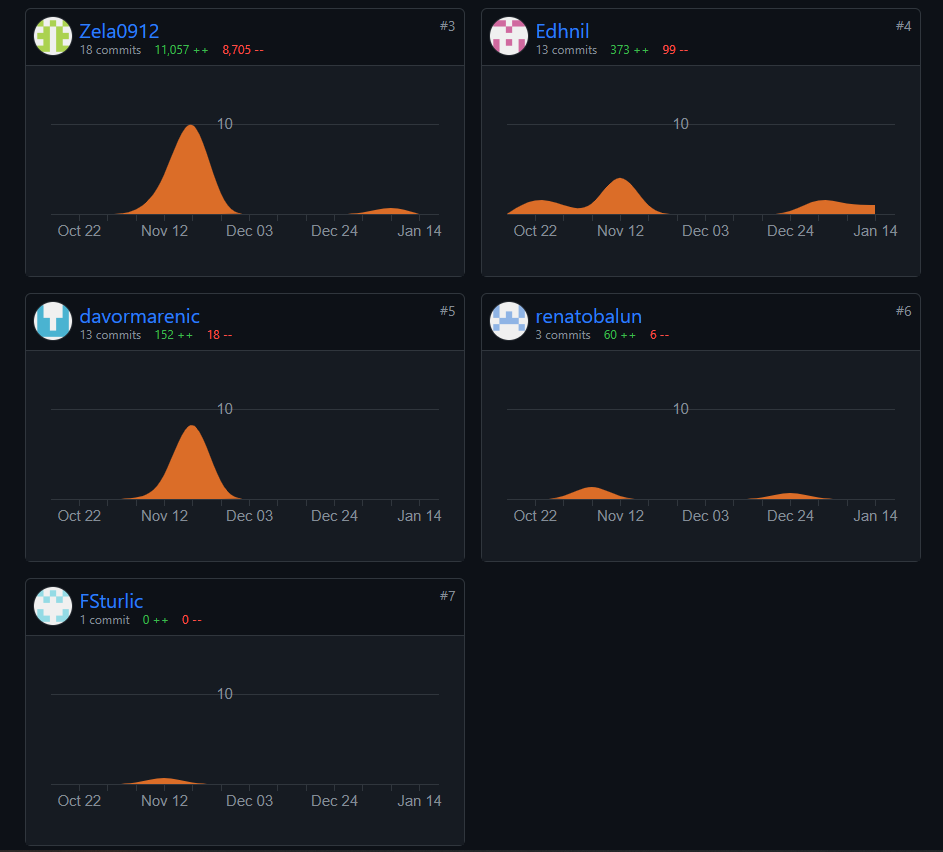
\includegraphics[width=\textwidth]{slike/d2.PNG} %veličina u odnosu na širinu linije
			\centering
			\caption{Graf GitHub aktivnosti}
			\label{fig:d2}
		\end{figure}
		
		\eject
		
	


\end{document} %naredbe i tekst nakon ove naredbe ne ulaze u izgrađen dokument 


